\documentclass[11pt]{article}
\pdfinfoomitdate=1
\pdftrailerid{}
\pdfsuppressptexinfo=15
\usepackage[T1]{fontenc}
\usepackage{lmodern}
\usepackage[margin=1in]{geometry}
\usepackage{amsmath,amssymb,amsthm,mathtools}
\usepackage{microtype}
\usepackage{enumitem}
\usepackage{booktabs}
\usepackage{tikz}
\usetikzlibrary{arrows.meta,positioning}
\usepackage{xcolor}
\usepackage{hyperref}
\hypersetup{colorlinks=true,linkcolor=blue!50!black,citecolor=blue!50!black,urlcolor=blue!50!black,
  pdftitle={A power saving for square-difference-free sets},pdfauthor={OpenAI}}
\usepackage[capitalise,noabbrev]{cleveref}
\numberwithin{equation}{section}
\newtheorem{theorem}{Theorem}[section]
\newtheorem{proposition}[theorem]{Proposition}
\newtheorem{lemma}[theorem]{Lemma}
\newtheorem{corollary}[theorem]{Corollary}
\theoremstyle{definition}
\newtheorem{definition}[theorem]{Definition}
\theoremstyle{remark}
\newtheorem{remark}[theorem]{Remark}
\newcommand{\E}{\mathbb E}
\renewcommand{\P}{\mathbb P}
\newcommand{\R}{\mathbb R}
\newcommand{\C}{\mathbb C}
\newcommand{\F}{\mathbb F}
\newcommand{\Z}{\mathbb Z}
\newcommand{\N}{\mathbb N}
\DeclareMathOperator{\supp}{supp}
\DeclareMathOperator{\lcm}{lcm}
\title{A power saving for square-difference-free sets}
\author{OpenAI}
\date{September 24, 2026}
\begin{document}
\maketitle
\begin{abstract}
We prove that there are absolute constants $c>0$ and $C<\infty$ such that
every set $A\subseteq\{1,\ldots,N\}$ with no nonzero square difference
satisfies $|A|\le C N^{1-c}$. This answers the fixed-power question posed
by Green and Sawhney.
\end{abstract}
\tableofcontents
\section{Introduction}
\label{sec:introduction}

For a positive integer $N$, write $[N]=\{1,\ldots,N\}$. A set
$A\subseteq[N]$ is \emph{square-difference-free} if
\[
 (A-A)\cap\{m^2:m\in\N,\ m\ge1\}=\varnothing.
\]
Thus the restriction concerns differences in the integers. Define
\[
 s(N)=\max\{|A|:A\subseteq[N]\text{ is square-difference-free}\}.
\]
Our main result is a fixed power saving in this extremal problem.

\begin{theorem}
\label{thm:main}
There are absolute constants $c>0$ and $C<\infty$ such that, for every
integer $N\ge1$ and every square-difference-free set $A\subseteq[N]$,
\[
 |A|\le C N^{1-c}.
\]
Equivalently, every subset of $[N]$ larger than $C N^{1-c}$ contains
distinct elements whose absolute difference is the square of a positive
integer.
\end{theorem}

The exponent obtained here is positive and absolute, but extremely small.
The argument does not yield a useful numerical value or an optimal exponent.
All finite constructions in the proof are fixed independently of $N$ and
$A$; their size affects the constants and the exponent.

\begin{remark}[Square-difference colorings]
Theorem~\ref{thm:main} gives a polynomial bound for the classical
square-difference coloring problem~\cite[Section~4]{BeigelGasarch2008}.
Fix its constants $c,C$, reducing $c$ so that $0<c<1$ if necessary.
Whenever integers $r,N\ge1$ satisfy $N>(Cr)^{1/c}$, every $r$-coloring
of $[N]$ has same-colored elements $a,a+d^2$ with $d\ge1$.
Indeed, a largest color class has size at least $N/r>C N^{1-c}$.
Only the two endpoints must share a color; no color restriction is
imposed on $d$. Equivalently, if $G_N$ is the graph on $[N]$ joining
distinct integers whose absolute difference is a square, then
\[
 \chi(G_N)\ge \frac{N}{s(N)}\ge C^{-1}N^c,
\]
since its independent sets are exactly the square-difference-free sets.
\end{remark}

\subsection{Previous work}

The problem originates in a question of Lov\'asz.
Furstenberg~\cite[Theorem~1.2]{Furstenberg1977} and S\'ark\"ozy~\cite{Sarkozy1978I}
proved independently that $s(N)=o(N)$, using ergodic theory and the
circle method, respectively. S\'ark\"ozy's quantitative estimate has the form
$s(N)\le N/(\log N)^{1/3+o(1)}$; see also the historical account
in~\cite{BloomMaynard2022}. Pintz, Steiger and
Szemer\'edi~\cite[Theorem~1]{PSS1988} strengthened this to
\[
 s(N)\ll \frac{N}{(\log N)^{c_{\rm PSS}\log\log\log\log N}}
\]
for an absolute $c_{\rm PSS}>0$. Their argument combines concentration on
arithmetic progressions with an iteration that increases the collection
of large Fourier coefficients. Bloom and Maynard~\cite{BloomMaynard2022}
subsequently obtained
\[
 s(N)\ll \frac{N}{(\log N)^{c_{\rm BM}\log\log\log N}}
\]
for an absolute $c_{\rm BM}>0$, using bounds for the additive energy of
rational numbers with small denominators to improve the density-increment
argument.


Green and Sawhney~\cite[Theorem~1.1]{GreenSawhney2025} prove
\[
 s(N)\ll N\exp\bigl(-c_1\sqrt{\log N}\bigr)
\]
for an absolute $c_1>0$. Their arithmetic level-$d$ inequality transfers
product-space hypercontractive estimates to rational Fourier coefficients.
Theorem~\ref{thm:main} answers affirmatively the fixed-power question
posed in~\cite[Section~1.1]{GreenSawhney2025}.
Adajar et al.~\cite[Theorem~1.1]{AdajarEtAl2026} extend the arithmetic
level-$d$ approach to fixed integer polynomials having a root modulo
every positive integer. For degree at least two they obtain a density
saving $\exp(-c(\log N)^\mu)$ for every fixed $0<\mu<1/2$, with
constants depending on the polynomial and $\mu$.

In the opposite direction, Ruzsa~\cite[Theorems~1 and~2]{Ruzsa1984}
constructed square-difference-free sets of size
$\gg N^{\gamma_0}$, where
\[
 \gamma_0=\frac12\left(1+\frac{\log 7}{\log 65}\right)
          =0.733077\ldots.
\]
His construction uses a set of residues with no square differences
modulo a squarefree integer to restrict selected digits of an integer
expansion. Beigel and Gasarch~\cite[Lemma~3.6 and the proof of Theorem~3.7]{BeigelGasarch2008} and
Lewko~\cite[Theorem~3]{Lewko2015} obtained the improved exponent
\[
 \gamma_1=\frac12\left(1+\frac{\log 12}{\log 205}\right)
          =0.733411797\ldots
\]
by exhibiting suitable sets of twelve residues modulo $205$.
Krachun's construction~\cite[Theorem~1]{Krachun2026} passes the
three-quarter threshold and gives
\[
 \liminf_{N\to\infty}\frac{\log s(N)}{\log N}
 \ge 0.752796455874514\ldots.
\]
A substantial gap remains between this lower exponent and the upper
exponent $1-c$ in Theorem~\ref{thm:main}.

Reflection positivity yields multilinear inequalities through the chessboard
method of Fr\"ohlich and Lieb~\cite[Theorem~2.2]{FrohlichLieb1978} and its
abstract formulation by Fr\"ohlich, Israel, Lieb and
Simon~\cite[Theorem~4.1]{FILS1978ReflectionI}.
Hatami~\cite[Theorem~2.8 of the arXiv version]{Hatami2010} characterizes
graph seminorms through mixed H\"older inequalities. Conlon and
Lee~\cite[Theorems~1.2 and~1.3]{ConlonLee2017Reflection} use finite
reflection groups to obtain such inequalities for absolute-value inputs,
and also for real-valued inputs when the two defining sets of simple
reflections are disjoint.
The signed mixed inequality is a classical feature of the chessboard
method; its role here is to permit Fourier lifts that can change sign.
We construct a finite-field probability law with the particular cycle
support, reflection positivity and conditional mixing needed for the
integer problem, and prove the signed inequality for that law directly.

The rational-frequency energy estimates of Bloom and
Maynard~\cite{BloomMaynard2022} and the product-space methods of Green and
Sawhney~\cite{GreenSawhney2025} are methodological precedents for the
arithmetic part. The argument retains rational Fourier analysis and
rescaling along square-step progressions. Here the quantity compared
between scales is a multilinear functional of a signed Fourier lift.

\subsection{Outline of the proof}

The proof constructs a nonnegative quantity that dominates a fixed power
of the density, and then proves that this quantity decreases by a power
of the interval length. The comparison with shorter intervals is available
for every residue specification. A separate estimate makes a fixed positive
proportion of those specifications negligible; these two estimates produce
the contraction.

Here is the quantity to be controlled. Choose a fixed even integer $d$
and a fixed set $V$ of $d$ labels. For a finite set $\mathcal P$ of sufficiently
large primes, put $X_{\mathcal P}=\prod_{p\in\mathcal P}\F_p$.
We will construct a probability law for a tuple $(z_v)_{v\in V}$ in
$X_{\mathcal P}$, and for a real function $g$ on this space define
\[
 Z_{\mathcal P}(g)=\E\prod_{v\in V}g(z_v).
\]
Its $d$-th root will be a seminorm satisfying
$|\E g|\le Z_{\mathcal P}(g)^{1/d}$. To apply it to $A\subseteq[N]$,
take $\mathcal P$ to be the primes between a fixed threshold $P$ and
$N^\beta$, where $\beta>0$ is fixed and small. Let $G$ retain the
rational Fourier coefficients of $1_A$ at frequencies of squarefree
reduced denominator at most $N^\beta$ whose prime factors all belong
to $\mathcal P$, including the zero frequency.
Section~\ref{sec:lift-moments} defines this \emph{Fourier lift} precisely.
It is real and its mean is exactly $|A|/N$, although its values may have
either sign. With these choices, write $Y(N,A)=Z_{\mathcal P}(G)$.
The seminorm bound gives
\[
 (|A|/N)^d\le Y(N,A).
\]
Thus a fixed power decay for $Y$ proves the theorem.

The tuple law is constructed separately over each prime field, then
multiplied over the primes, collecting the field labels into vectors
$z_v\in X_{\mathcal P}$. Every individual field label is uniform.
The law has two further properties with distinct purposes.
First, it is reflection positive: specified involutions of $V$ exchange
two halves, and the matrix coupling the half-tuples is symmetric positive
semidefinite. Repeated Cauchy--Schwarz across these cuts proves the signed
mixed inequality and seminorm bound
(Proposition~\ref{prop:signed-holder}). Second, outside a part of mass
at most $p^{-4}$, a designated directed cycle of $24$ labels has nonzero
square differences in $\F_p$, and each of its edge pairs is uniform
among pairs with such a difference. This exact pair law supplies the
arithmetic input below. The full reflection-positive law and its normalized
nonexceptional part also satisfy conditional mixing, which makes inputs
with large Fourier denominators negligible
(Lemma~\ref{lem:conductor-decay}). Section~\ref{sec:tuple-laws} constructs
these laws from the graph estimates of Section~\ref{sec:finite-field-graphs}.

The approximation errors require control of signed lifts beyond their
means. Every fixed moment of $G$ grows more slowly than any fixed positive
power of $N$, uniformly in the prime set and in every retained family of
complete denominator classes. Lemma~\ref{lem:lift-moments} proves this
by a conditional square-function estimate and symmetrization. The same
bounds, with an explicit fiber-size cost, remain available after specifying
some prime coordinates. Combined with conductor decay, they justify the
Fourier truncations used in both estimates that follow.

For the change of scale, fixing prime coordinates whose product is at
most a sufficiently small fixed power of $N$ makes the low Fourier
coefficients exact averages on an integer residue class modulo an integer
$D$. Splitting that class into progressions of common difference $D^2$
and rescaling preserves square-difference avoidance: a square difference
in a rescaled set would give a square difference in $A$.
The seminorm's square-affine symmetries therefore compare the specialized
functional with the same functional at length $\lceil N/D^2\rceil$,
up to a factor tending to one and a power-decaying error
(Proposition~\ref{prop:scale-transfer}). This comparison applies to all
specified residues, without using the exceptional splitting.

The arithmetic cancellation uses the normalized nonexceptional prime laws.
Set aside the finitely many primes below the tuple-law threshold, together
with modulus $8$, in one fixed modulus $M_0$. Independently choose one
residue modulo $M_0$ for each slot. A fixed positive proportion of these
assignments has strict square differences along the designated cycle:
they are $1$ modulo $8$ and nonzero squares modulo every odd prime
dividing $M_0$.
For such an assignment, divide $[N]$ into ordered intervals. Unless all
cycle slots choose the same interval, one directed edge goes from an
earlier interval to a later one. Truncating and expanding the other slots
reduces its contribution to the selected pair law. A signed kernel
supported on actual shifts $m^2$ then bounds that contribution using the
absence of integer square differences
(Propositions~\ref{prop:square-kernel} and~\ref{prop:nonexceptional-contraction}).
The event that all cycle slots choose one interval is itself small.

Finally, Section~\ref{sec:induction} expands the exceptional submeasures
by inclusion--exclusion. Exceptional prime sets of large product are
bounded directly by moment estimates. A smaller exceptional prime set
with product $q_B$ leads to the shorter scale approximately $N/(M_0q_B)^2$.
Its mass remains summable even after multiplication by $q_B$; this absorbs
the factor $q_B^{2a_0}$ incurred by a sufficiently small proposed decay
exponent $a_0$. Combining this bound with the universal scale comparison
and the cancellation on a positive proportion of small-residue assignments
gives a strict weighted recurrence. Induction proves
$Y(N,A)\ll N^{-a_0}$, and the density inequality above gives
Theorem~\ref{thm:main} with $c=a_0/d$.
Figure~\ref{fig:proof-map} records the principal inputs to this assembly.
\begin{figure}[htbp]
\centering
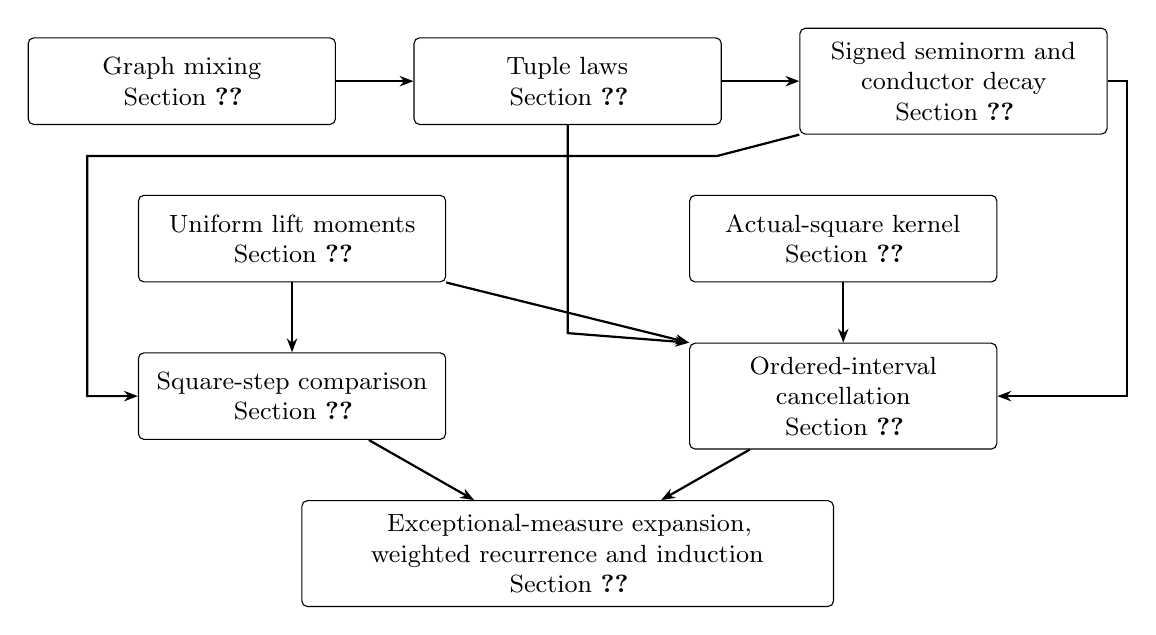
\begin{tikzpicture}[
  box/.style={draw,rounded corners=2pt,align=center,font=\small,
              text width=3.55cm,minimum height=1.1cm,inner sep=5pt},
  arr/.style={-{Stealth[length=5pt]},thick},x=1cm,y=1cm]
\node[box] (graph) at (-4.9,0) {Graph mixing\\Section~\ref{sec:finite-field-graphs}};
\node[box] (tuple) at (0,0) {Tuple laws\\Section~\ref{sec:tuple-laws}};
\node[box] (functional) at (4.9,0) {Signed seminorm and\\conductor decay\\Section~\ref{sec:functional}};
\node[box] (moments) at (-3.5,-2) {Uniform lift moments\\Section~\ref{sec:lift-moments}};
\node[box] (kernel) at (3.5,-2) {Actual-square kernel\\Section~\ref{sec:square-kernel}};
\node[box] (transfer) at (-3.5,-4) {Square-step comparison\\Section~\ref{sec:scale-transfer}};
\node[box] (cancel) at (3.5,-4) {Ordered-interval cancellation\\Section~\ref{sec:ordered-contraction}};
\node[box,text width=6.4cm] (induct) at (0,-6) {Exceptional-measure expansion,\\weighted recurrence and induction\\Section~\ref{sec:induction}};
\draw[arr] (graph) -- (tuple);
\draw[arr] (tuple) -- (functional);
\draw[arr] (moments) -- (transfer);
\draw[arr] (moments.south east) -- (cancel.north west);
\draw[arr] (kernel) -- (cancel);
\draw[arr] (functional.east) -- (7.1,0) -- (7.1,-4) -- (cancel.east);
\draw[arr] (functional.south west) -- (1.9,-.95) -- (-6.1,-.95) -- (-6.1,-4) -- (transfer.west);
\draw[arr] (tuple.south) -- (0,-1.25) -- (0,-3.2) -- (cancel.north west);
\draw[arr] (transfer) -- (induct);
\draw[arr] (cancel) -- (induct);
\end{tikzpicture}
\caption{Principal proof inputs. The full tuple law supplies reflection
positivity for the signed seminorm; the normalized nonexceptional law
supplies the strict-square pair law for cancellation. Both have the
conditional mixing used in conductor decay. The two lower branches are
combined only in the weighted recurrence. Arrows indicate dependencies,
not equivalences.}
\label{fig:proof-map}
\end{figure}


\subsection{Conventions}

All averages on finite sets are with respect to uniform probability
measure unless another measure is displayed. All $L^r$ norms of functions
on $X_{\mathcal P}$ use its uniform product measure. Empty products are
$1$; the product over an empty prime set is a one-point space. We write
$e(t)=\exp(2\pi i t)$ and identify rational frequencies modulo $1$.
The \emph{conductor} of a rational frequency is its reduced positive
denominator; the conductor of $0$ is $1$.

For nonnegative quantities, $U\ll V$ means $U\le C V$ for a constant
with the dependencies stated in context. A uniform bound $U=N^{o(1)}$
means that for every $\varepsilon>0$ there is a constant
$C_\varepsilon$ such that $U\le C_\varepsilon N^\varepsilon$ for all
allowed data. Fixed tuple sizes and fixed moment orders may affect
$C_\varepsilon$; sets, intervals, chosen residues and retained frequency
families may not. All final choices of parameters are made independently
of $N$ and $A$.

\section{Finite-field square constraints}
\label{sec:finite-field-graphs}

This section controls systems of square constraints on independent field
variables.  A single constraint is close to a constant kernel in operator
norm.  Replacing constraints one at a time then counts any fixed directed
graph without loops or opposite edges.  Applying this count to a four-cycle
of two lists gives the operator estimate needed for the tuple measures.

Throughout, finite sets carry uniform probability measure, and
\(e(t)=\exp(2\pi i t)\).  For an odd prime \(p\), write
\[
 Q_p^*=\{u^2:u\in\mathbb F_p^\times\},
 \qquad
 A_p(t)=1_{Q_p^*}(t),
 \qquad
 \delta_p=\frac{\sqrt p+1}{2p}\le p^{-1/2}.
\]
For finite sets \(X,Y\), the operator associated with a kernel
\(K:X\times Y\to\mathbb R\) is
\[
 T_K f(x)=\mathbb E_{y\in Y}K(x,y)f(y).
\]
We use \(\|K\|_{\mathrm{op}}\) to mean the norm of \(T_K\) from
\(L^2(Y)\) to \(L^2(X)\).  A constant kernel \(c\) therefore denotes
the operator \(f\mapsto c\,\mathbb E f\).

\begin{lemma}[Counting directed square constraints]
\label{lem:graph-count}
Let \(p\) be an odd prime and let \(G=(W,E)\) be a finite directed graph
with no loops and at most one edge on each unordered pair of distinct
vertices.  Put \(m=|E|\), and let \((z_w)_{w\in W}\) be independent
uniform elements of \(\mathbb F_p\).  Then
\[
 \left|
 \mathbb E\prod_{(u,v)\in E}A_p(z_v-z_u)-2^{-m}
 \right|
 \le m\delta_p.
\]
The assertion includes the empty graph, whose product is \(1\).
\end{lemma}

\begin{proof}
We first show that the kernel
\(b_p(x,y)=A_p(y-x)-1/2\) has operator norm at most \(\delta_p\).
The characters \(x\mapsto e(kx/p)\), \(k\in\mathbb F_p\), are an
orthonormal eigenbasis.  The constant eigenvalue is
\[
 \frac{|Q_p^*|}{p}-\frac12=-\frac1{2p}.
\]
For \(k\ne0\), put \(G_p(k)=\sum_{u\in\mathbb F_p}e(ku^2/p)\).
The corresponding eigenvalue is
\[
 \frac1p\sum_{t\in Q_p^*}e(kt/p)
 =\frac{G_p(k)-1}{2p}.
\]
Here the subtraction of \(1\) removes the zero square, and division
by \(2\) removes the multiplicity of every nonzero square.  Since
\((u,v)\mapsto(u-v,u+v)\) is a bijection on \(\mathbb F_p^2\),
\[
 |G_p(k)|^2
 =\sum_{u,v\in\mathbb F_p}e\bigl(k(u^2-v^2)/p\bigr)
 =\sum_{a,b\in\mathbb F_p}e(kab/p)
 =p.
\]
Thus all eigenvalues have absolute value at most \(\delta_p\).
In particular,
\begin{equation}
 \left|
 \mathbb E_{x,y} f(x)g(y)\bigl(A_p(y-x)-\tfrac12\bigr)
 \right|
 \le\delta_p\|f\|_2\|g\|_2.
 \label{eq:single-square-mixing}
\end{equation}
The same bound holds with \(x-y\) in place of \(y-x\), since the
transposed operator has the same norm.

Now replace the \(m\) edge indicators one at a time by \(1/2\).
In a telescoping error for an edge \((u,v)\), fix every variable
except \(z_u,z_v\).  No other edge has both these endpoints.
Consequently all the other factors separate as
\(C f(z_u)g(z_v)\), where \(|C|,|f|,|g|\le1\).
Equation~\eqref{eq:single-square-mixing} bounds the conditional error
by \(\delta_p\).  Averaging the fixed variables and summing over
the edges proves the assertion.
\end{proof}

We next divide the variables into two independent lists.  Only
constraints between the lists enter the following kernel; constraints
within either list must be treated separately.

\begin{lemma}[Mixing between two lists]
\label{lem:list-mixing}
Let \(I,J\) be finite disjoint sets, and let \(G\) be a directed graph
on \(I\sqcup J\) whose \(m\) edges all join \(I\) to \(J\), with at
most one edge on each unordered pair.  The directions may vary from
edge to edge.  For
\(x\in\mathbb F_p^I\), \(y\in\mathbb F_p^J\), write \(z_i=x_i\) for
\(i\in I\), \(z_j=y_j\) for \(j\in J\), and set
\[
 K(x,y)=\prod_{(u,v)\in E(G)}A_p(z_v-z_u).
\]
Then
\begin{equation}
 \|K-2^{-m}\|_{\mathrm{op}}
 \le (32m)^{1/4}p^{-1/8}.
 \label{eq:list-mixing}
\end{equation}
For \(m=0\), both sides are zero.  In particular, the implied
constant for any fixed pair of lists is independent of \(p\).
\end{lemma}

\begin{proof}
Put \(c=2^{-m}\) and \(B=K-c\).  With respect to the normalized
point-mass bases, \(T_B\) has matrix entries
\(B(x,y)/\sqrt{|\mathbb F_p^I|\,|\mathbb F_p^J|}\).
If \(s_r\) are its singular values, then
\begin{align}
 \|B\|_{\mathrm{op}}^4
 &\le \sum_r s_r^4
 =\operatorname{tr}\bigl((T_BT_B^*)^2\bigr) \notag\\
 &=\mathbb E_{x^0,x^1,y^0,y^1}
 B(x^0,y^0)B(x^0,y^1)B(x^1,y^0)B(x^1,y^1),
 \label{eq:list-four-cycle}
\end{align}
where the four lists are independent and uniform.  The kernel is
real, so no conjugates appear in the last expression.

Let \(\Omega=\{0,1\}^2\).  Expanding the last line gives
\[
 \sum_{F\subseteq\Omega}(-c)^{4-|F|}
 \mathbb E\prod_{(a,b)\in F}K(x^a,y^b).
\]
For each \(F\), its product is the constraint indicator of a graph
on
\[
 (I\times\{0,1\})\sqcup(J\times\{0,1\}).
\]
Every base edge between \(i\in I\) and \(j\in J\) is copied, in its
original direction, between \((i,a)\) and \((j,b)\) for every
\((a,b)\in F\).  The two endpoints determine the base unordered
pair and the corner \((a,b)\).  Hence this graph has no loops or
repeated unordered edges, and has exactly \(m|F|\) edges.
Lemma~\ref{lem:graph-count} therefore gives
\[
 \mathbb E\prod_{(a,b)\in F}K(x^a,y^b)
 =c^{|F|}+E_F,
 \qquad |E_F|\le m|F|\delta_p.
\]
The main terms sum to \((c-c)^4=0\).  The remaining terms have
absolute value at most
\[
 m\delta_p\sum_{t=0}^4\binom4t t c^{4-t}
 =4m(1+c)^3\delta_p
 \le32m p^{-1/2}.
\]
Combining this with \eqref{eq:list-four-cycle} and taking fourth
roots proves \eqref{eq:list-mixing}.
\end{proof}

\section{Finite reflection-positive probability laws}
\label{sec:tuple-laws}

We construct probability laws on a fixed set of field labels.  Their
nonexceptional parts enforce a directed cycle of square differences.
The full laws also satisfy positivity across a family of reflection cuts.
To obtain both properties, we add a finite hierarchy of measures in which
successively more blocks of the index set are marked.  A marked block
provides a positive quadratic form that dominates the small negative part
at the corresponding unmarked cut.

\subsection{The index set and the required properties}

Fix the integers
\begin{equation}
 h=24,\qquad t_0=80,\qquad \ell=2t_0+1=161.
 \label{eq:tuple-fixed-parameters}
\end{equation}
Let \(\Pi\) be the set of permutation words on \([h]=\{1,\ldots,h\}\),
viewed as bijections from positions to symbols.  Write
\[
 K=h!,\qquad r=K/2,\qquad V=\Pi^\ell,\qquad d=|V|=K^\ell,
 \qquad n=d/2.
\]
The coordinates of a vertex \(v\in V\) are called its blocks.
Fix a cycle \(c\) of length \(h\) on the positions.  Composition on
the right, \(w\mapsto wc\), cyclically shifts a word.  Define
\(v_0,\ldots,v_{h-1}\in V\) by giving every block of \(v_j\) the
word \(c^j\), and put \(v_h=v_0\).

A reflection is specified by a block \(b\in[\ell]\) and two
distinct symbols \(\alpha,\beta\).  It acts on \(V\) by swapping
these symbols on the left in block \(b\); denote this involution by
\(\theta\).  Its associated cut is
\[
 V_+=\{v:\alpha\text{ precedes }\beta\text{ in block }b\},
 \qquad V_-=\theta V_+.
\]
The reflection has no fixed vertices, and both halves have size \(n\).

For a finite alphabet \(X\), a measure \(\nu\) on \(X^V\) defines
a matrix whose row index is \((z_v)_{v\in V_+}\) and whose column
index is \((z_{\theta v})_{v\in V_+}\).  We say that \(\nu\) is
\emph{reflection positive} if this matrix is symmetric positive
semidefinite for every cut above.  Equivalently, symmetry holds and
\[
 \int F((z_v)_{v\in V_+})F((z_{\theta v})_{v\in V_+})\,d\nu(z)
 \ge0
\]
for every real function \(F:X^{V_+}\to\mathbb R\).

Recall that \(Q_p^*=\{u^2:u\in\mathbb F_p^\times\}\) for an odd
prime \(p\).  The following proposition summarizes the construction.

\begin{proposition}[Tuple laws]
\label{prop:tuple-laws}
There is an absolute integer \(P\) such that, for every prime
\(p\ge P\), there are a probability measure \(\mu_p\) on
\(\mathbb F_p^V\) and a nonnegative submeasure \(\varepsilon_p\le\mu_p\)
whose mass satisfies
\[
 \eta_p=\varepsilon_p(\mathbb F_p^V)\le p^{-4}.
\]
Writing
\[
 \mu_p^\circ=\frac{\mu_p-\varepsilon_p}{1-\eta_p},
\]
the following properties hold.
\begin{enumerate}
\item The full law \(\mu_p\) is reflection positive.  Both
\(\mu_p\) and \(\varepsilon_p\) are invariant under simultaneous
changes \(z_v\mapsto qz_v+a\), where \(a\in\mathbb F_p\) and
\(q\in Q_p^*\).  Every single-label marginal of \(\mu_p\) and
\(\mu_p^\circ\) is uniform on \(\mathbb F_p\).
\item On the support of
\(\mu_p^\circ\),
\[
 z_{v_{j+1}}-z_{v_j}\in Q_p^*\qquad(0\le j<h).
\]
The marginal of each ordered pair \((z_{v_j},z_{v_{j+1}})\) under
\(\mu_p^\circ\) is uniform on
\(\{(x,y):y-x\in Q_p^*\}\).
\item Put \(\gamma=1/64\).  For either \(\rho_p=\mu_p\) or
\(\rho_p=\mu_p^\circ\), every \(v\in V\), and every
\(f:\mathbb F_p\to\mathbb C\) with uniform mean zero,
\begin{equation}
 \left\|\mathbb E_{\rho_p}
 \bigl[f(z_v)\mid(z_w)_{w\ne v}\bigr]\right\|_2
 \le p^{-\gamma}\|f\|_2.
 \label{eq:tuple-conditional-bound}
\end{equation}
The norm on the left uses the other-label marginal of \(\rho_p\);
the norm on the right uses uniform measure on \(\mathbb F_p\).
\end{enumerate}
\end{proposition}

The cycle length $h$ and the total tuple size $d$ are fixed before any
prime or integer interval is chosen. Thus constants depending on this
finite construction remain absolute throughout the proof.

The construction and reflection estimates are given below.
Lemma~\ref{lem:conditional-mixing} will establish the final assertion
and the precise pair marginal.

\subsection{Measures with marked blocks}

Start with one independent uniform label at each vertex of $V$. Require a
strict square difference from $v$ to $w$ whenever $w_a=v_ac$ in at least
$t_0+1$ blocks. In particular these constraints include every edge of the
designated cycle. Multiplying the uniform product measure by the indicator
of all these constraints gives the leading component, an unnormalized
measure. Its cut matrices need not be positive semidefinite; the graph
estimates control their negative parts.

To compensate for those negative parts, we introduce components in which
vertices that agree outside a set of marked blocks draw their labels from
a common list. A positive weight couples their choices of list entries.
Marking a block then provides a lower bound at its reflection cuts, while
leaving enough unmarked blocks to retain the cycle constraints until the
last level. The following definitions implement this construction.

For \(S\subseteq[\ell]\) with \(s=|S|\le t_0+1\), regard the
blocks in \(S\) as marked; blocks outside \(S\) are called
\emph{clean}. We call the marking nonterminal if $s\le t_0$ and
terminal if $s=t_0+1$. The terminal components will form the exceptional
measure. Let
\[
 U_S=\Pi^{[\ell]\setminus S},\qquad m_s=r^s,
\]
and let \(u_S:V\to U_S\) forget the marked blocks.  At every
address \(u\in U_S\), choose a list
\((Y_{u,i})_{i\in[m_s]}\) of independent uniform elements of
\(\mathbb F_p\).  All lists are independent.  The total number of
list entries is
\begin{equation}
 |U_S|m_s=K^{\ell-s}r^s=d/2^s\le d.
 \label{eq:tuple-list-count}
\end{equation}

For \(s\le t_0\), draw an address edge \(u\to u'\) exactly when
\begin{equation}
 \#\{a\notin S:u'_a=u_ac\}\ge\ell-t_0=t_0+1.
 \label{eq:tuple-address-edge}
\end{equation}
For each such edge require
\begin{equation}
 Y_{u',i'}-Y_{u,i}\in Q_p^*
 \quad\text{for all }i,i'\in[m_s].
 \label{eq:tuple-list-constraint}
\end{equation}
Let \(I_S(Y)\) be the indicator of all these conditions.
For \(s=t_0+1\), impose no conditions and set \(I_S=1\).
The graph on list entries defined by
\eqref{eq:tuple-list-constraint} will be denoted by \(\mathcal G_S\).

There are no loops in the address graph: a permutation word cannot
equal its nontrivial position shift.  Nor can both directions occur
between two addresses.  Indeed, the clean blocks counted for the two
directions are disjoint, since a block counted for both would imply
\(c^2=1\).  Their combined required size is \(2(t_0+1)>\ell\),
which is impossible.  Each unordered pair of list entries therefore
supports at most one directed edge in \(\mathcal G_S\).
Lemma~\ref{lem:graph-count} applies to this graph and all its induced
subgraphs.

Set
\[
 \delta=\frac1{10h^2}.
\]
For distinct \(v,w\in V\), define a symmetric interaction
\(H^S_{vw}\) as follows.  It is zero unless \(v,w\) differ by a
symbol transposition in exactly one marked block.  In that case,
if the positions of the swapped symbols have gap \(g\), put
\(H^S_{vw}=\delta^g\).  Independently of the lists, choose all
indices \(j_v\in[m_s]\) uniformly and independently, and give their
joint distribution the unnormalized weight
\begin{equation}
 W_S(j)=\exp\left(
 \sum_{\{v,w\}\subseteq V}H^S_{vw}1_{\{j_v=j_w\}}\right).
 \label{eq:tuple-index-weight}
\end{equation}
Every sum over \(\{v,w\}\) is over unordered pairs of distinct
vertices, so each interaction is counted once.

Define the finite measure \(\nu_{p,S}\) by the identity
\begin{equation}
 \int G(z)\,d\nu_{p,S}(z)
 =\mathbb E_Y\mathbb E_j I_S(Y)W_S(j)
 G\bigl((Y_{u_S(v),j_v})_{v\in V}\bigr)
 \label{eq:tuple-component-law}
\end{equation}
for all functions \(G\) on \(\mathbb F_p^V\).  Both expectations
on the right are uniform probability averages.  In particular,
\(\nu_{p,S}\) has not been normalized to have mass one.
We also write \(\nu(1)\) for the total mass of a finite measure \(\nu\).

Each vertex has at most \(s\binom h2\) neighbors with nonzero
interaction, and each interaction is at most \(\delta\).  Thus,
with the fixed constant
\begin{equation}
 B=\exp\left(\frac{d(t_0+1)\binom h2\delta}{2}\right),
 \label{eq:tuple-weight-bound}
\end{equation}
we have
\begin{equation}
 1\le W_S(j)\le B,\qquad \nu_{p,S}(\mathbb F_p^V)\le B.
 \label{eq:tuple-component-mass-upper}
\end{equation}

For a cut with reflection \(\theta\), define the quadratic form
\begin{equation}
 Q_{p,S}^{b}(F)=
 \int F((z_v)_{v\in V_+})
 F((z_{\theta v})_{v\in V_+})\,d\nu_{p,S}(z).
 \label{eq:tuple-cut-form}
\end{equation}
The notation suppresses the two symbols that specify the cut.
Every component has a symmetric matrix at every cut, as we now verify.

\begin{lemma}[Symmetry of the component matrices]
\label{lem:tuple-component-symmetry}
For every allowed mark set \(S\) and every reflection \(\theta\),
the measure \(\nu_{p,S}\) is invariant under the permutation
\((z_v)\mapsto(z_{\theta v})\).  Its matrix at that cut is symmetric.
\end{lemma}

\begin{proof}
The array \(H^S\) is invariant under simultaneous application of
\(\theta\) to both endpoints.  In the reflected block, conjugating
a symbol transposition changes only the names of the swapped symbols,
not their positional gap.  Interactions in other blocks retain their
gap as well.  Hence relabeling indices by \(j_v\mapsto j_{\theta v}\)
preserves their uniform law and weight.

If the reflected block is marked, \(u_S(\theta v)=u_S(v)\), so
no relabeling of lists is needed.  If it is unmarked, \(\theta\)
acts on addresses.  Left symbol permutations commute with the right
position shift \(c\); therefore it preserves the directed address
relation \eqref{eq:tuple-address-edge}, including its orientation.
Relabeling lists by this address involution preserves their uniform
law and \(I_S\).  In either case these bijections in
\eqref{eq:tuple-component-law} send the output label at \(v\) to
the label at \(\theta v\), proving invariance.  At the cut this
invariance exchanges the two matrix indices, which is symmetry.
\end{proof}

\subsection{Strict positivity at a marked cut}

The next estimate is the source of domination between successive
mark sets.  It must remain valid when different index assignments
produce identical field labels.

\begin{lemma}[Marked-cut lower bound]
\label{lem:marked-positive}
Put
\[
 \kappa=\frac9{10}\delta^{h-1},\qquad
 \lambda=(e^\kappa-1)^n,\qquad
 c_* =\lambda m_{t_0+1}^{-n}>0.
\]
For every \(S\) with \(|S|\le t_0+1\), every cut in a marked block
\(b\in S\), and every real \(F:\mathbb F_p^{V_+}\to\mathbb R\),
\begin{equation}
 Q_{p,S}^{b}(F)
 \ge \lambda m_s^{-n}\,
 \mathbb E_{Y,j_+}I_S(Y)
 F((Y_{u_S(v),j_v})_{v\in V_+})^2.
 \label{eq:tuple-marked-lower}
\end{equation}
Here the expectation uses all uniform lists and only the uniform
indices on \(V_+\).  In particular, the coefficient in
\eqref{eq:tuple-marked-lower} is at least \(c_*\), independently
of the prime and of the field-list values.
\end{lemma}

\begin{proof}
Index an \(n\times n\) matrix by \(x,y\in V_+\) and set
\[
 \mathsf A_{xy}=H^S_{x,\theta y}.
\]
The invariance of \(H^S\) used in
Lemma~\ref{lem:tuple-component-symmetry}, together with its symmetry,
gives \(\mathsf A_{xy}=\mathsf A_{yx}\).

Suppose the two cut symbols occupy positions \(i<j\) in the
reflected block of \(x\), and set \(g=j-i\).  The diagonal entry
is \(\mathsf A_{xx}=\delta^g\).  A transposition taking \(x\)
across the cut must act in this block and involve a cut symbol.
Apart from swapping the two cut symbols themselves, it must either
move the first symbol from \(i\) to a position \(k>j\), or move
the second from \(j\) to a position \(k<i\).  Its gap is therefore
at least \(g+1\).  There are fewer than \(h^2\) such transpositions,
so
\[
 \sum_{y\ne x}|\mathsf A_{xy}|
 \le h^2\delta^{g+1}=\frac1{10}\mathsf A_{xx}.
\]
For every real vector \(a\), using
\(2|a_xa_y|\le a_x^2+a_y^2\) gives
\begin{align}
 a^T\mathsf Aa
 &\ge\sum_x\left(\mathsf A_{xx}
       -\sum_{y\ne x}|\mathsf A_{xy}|\right)a_x^2\notag\\
 &\ge\frac9{10}\delta^{h-1}\sum_xa_x^2
 =\kappa\sum_xa_x^2.
 \label{eq:tuple-cross-interaction-lower}
\end{align}

Write \(m=m_s\) and \(\mathcal J=[m]^{V_+}\).  For
\(j\in\mathcal J\), define a vector with one nonzero coordinate
for each vertex \(x\in V_+\) by
\[
 u(j)=(1_{\{j_x=i\}})_{x\in V_+,\ i\in[m]}.
\]
Using the reflected indices on the minus side, the cross factor of
\eqref{eq:tuple-index-weight} is the matrix
\[
 \mathsf C(j,k)=
 \exp\bigl(u(j)^T(\mathsf A\otimes I_m)u(k)\bigr).
\]
Each unordered cross pair is uniquely \(\{x,\theta y\}\) with
\(x,y\in V_+\), so no extra factor of two appears in this formula.

By \eqref{eq:tuple-cross-interaction-lower},
\(\mathsf D=(\mathsf A-\kappa I_n)\otimes I_m\) is positive
semidefinite.  The matrix
\[
 \mathsf R(j,k)=\exp\bigl(u(j)^T\mathsf D u(k)\bigr)
\]
is positive semidefinite: after taking a square root of
\(\mathsf D\), the bilinear form is an inner product, and each
term of the exponential series is a Gram matrix of tensor powers
with a nonnegative coefficient.  The convergent sum is positive
semidefinite.  Moreover \(\mathsf R(j,j)\ge1\).

The remaining factor is
\[
 \mathsf E(j,k)=
 \exp\left(\kappa\sum_{x\in V_+}1_{\{j_x=k_x\}}\right).
\]
As a matrix this is
\[
 \mathsf E=\bigotimes_{x\in V_+}
 \bigl((e^\kappa-1)I_m+\mathbf1\mathbf1^T\bigr).
\]
Every factor dominates \((e^\kappa-1)I_m\), also for \(m=1\).
It follows that \(\mathsf E\) dominates \(\lambda I_{\mathcal J}\).
The entrywise product of positive semidefinite matrices is positive
semidefinite: if they are Gram matrices, the products of their
entries are the Gram matrix of pairwise tensor products.  Denoting
entrywise multiplication by \(\circ\), we therefore obtain
\begin{equation}
 \mathsf C
 = (\mathsf E-\lambda I_{\mathcal J})\circ\mathsf R
   +\lambda(I_{\mathcal J}\circ\mathsf R)
 \succeq\lambda I_{\mathcal J}.
 \label{eq:tuple-exponential-lower}
\end{equation}

The internal weight on the plus half is
\[
 a(j)=\exp\left(\sum_{\{x,y\}\subseteq V_+}
 H^S_{xy}1_{\{j_x=j_y\}}\right)\ge1.
\]
The reflected minus weight is the same function of its indices.
Thus the full index matrix is
\(\operatorname{diag}(a)\mathsf C\operatorname{diag}(a)\),
which still dominates \(\lambda I_{\mathcal J}\) by
\eqref{eq:tuple-exponential-lower}.

Fix the lists.  Since \(b\in S\), the two reflected vertices
\(v,\theta v\) have the same address.  Consequently both sides
of the quadratic form use the same vector
\[
 f_Y(j)=F((Y_{u_S(v),j_v})_{v\in V_+}).
\]
This vector may have repeated entries.  No injectivity of the map
from index assignments to field assignments is required for the
matrix lower bound.  Since \(|\mathcal J|=m^n\), the full uniform
index average is bounded below by
\[
 \lambda m^{-2n}\sum_{j\in\mathcal J}f_Y(j)^2
 =\lambda m^{-n}\mathbb E_{j\in\mathcal J}f_Y(j)^2.
\]
Multiply by \(I_S(Y)\) and average over the lists.  This proves
\eqref{eq:tuple-marked-lower}.  The stated uniform coefficient
follows from \(m_s\le m_{t_0+1}\).
\end{proof}

\subsection{The error at an unmarked cut}

At an unmarked cut, the lists themselves split into two independent
families.  Lemma~\ref{lem:list-mixing} controls the possible negative
part of the cut form.

\begin{lemma}[Unmarked-cut error]
\label{lem:unmarked-error}
Let \(b\notin S\) specify a cut and suppose \(s=|S|\le t_0\).
Let \(Y_+\) consist of the lists at plus addresses, and let
\(I_+(Y_+)\) impose only the constraints internal to those addresses.
For a real half-label function \(F\), put
\[
 D_{p,S}^{b}(F)=\mathbb E_{Y_+,j_+}I_+(Y_+)
 F((Y_{u_S(v),j_v})_{v\in V_+})^2.
\]
Then, with the fixed constant \(C_*=(32d^2)^{1/4}B^2\),
\begin{equation}
 Q_{p,S}^{b}(F)\ge-C_*p^{-1/8}D_{p,S}^{b}(F).
 \label{eq:tuple-unmarked-error}
\end{equation}
If instead \(s=t_0+1\), the form \(Q_{p,S}^{b}\) is nonnegative.
\end{lemma}

\begin{proof}
Use \(\theta\) to identify the minus-address list space with a
second copy of the plus-address space.  Symmetry of the directed
graph gives the factorization
\[
 I_S(Y_+,Y_-)=I_+(Y_+)I_+(Y_-)K_b(Y_+,Y_-),
\]
where \(K_b\) is the product of the constraints crossing the cut.
Its graph is bipartite, simple on unordered pairs, and may contain
both orientations on different pairs.  If it has \(e_b\) edges,
then \(e_b\le d^2\) by \eqref{eq:tuple-list-count}.
Lemma~\ref{lem:list-mixing} yields
\[
 \|K_b-2^{-e_b}\|_{\mathrm{op}}
 \le(32d^2)^{1/4}p^{-1/8}.
\]

Every nonzero index interaction changes a marked block, and so
preserves the unmarked word in block \(b\).  No such interaction
crosses the cut.  The index weight therefore factors as
\(W_+(j_+)W_+(j_-)\), with the same function on the reflected
halves and \(1\le W_+\le B\).  Set
\[
 G(Y_+)=I_+(Y_+)\mathbb E_{j_+}W_+(j_+)
 F((Y_{u_S(v),j_v})_{v\in V_+}).
\]
Then \(Q_{p,S}^{b}(F)=\langle G,T_{K_b}G\rangle\).
The constant kernel contributes the nonnegative quantity
\(2^{-e_b}(\mathbb E G)^2\).  Cauchy--Schwarz in the uniform index
average, followed by \(I_+^2=I_+\) and \(W_+\le B\), gives
\[
 \|G\|_2^2\le B^2D_{p,S}^{b}(F).
\]
The operator error proves \eqref{eq:tuple-unmarked-error}.
For \(s=t_0+1\), no field constraints are present, so the same
factorization gives exactly \(Q_{p,S}^{b}(F)=(\mathbb E G)^2\ge0\).
\end{proof}

\subsection{Domination and the reflection-positive mixture}

We now compare the two preceding lemmas.  Marking a further block
combines all its plus-side lists into one longer list.  The precise
length \(m_s=r^s\) ensures that this identification preserves the
uniform product distribution.

\begin{lemma}[Domination after marking a block]
\label{lem:tuple-marking-domination}
Let \(b\notin S\), \(|S|\le t_0\), and set
\(S'=S\cup\{b\}\).  For the cut in block \(b\) and every real
half-label function \(F\),
\begin{equation}
 Q_{p,S'}^{b}(F)\ge c_*r^{-n}D_{p,S}^{b}(F).
 \label{eq:tuple-marking-domination}
\end{equation}
Consequently the measure
\(\nu_{p,S}+p^{-1/16}\nu_{p,S'}\) has a positive semidefinite
matrix at this cut whenever
\begin{equation}
 p\ge P_{\mathrm{ref}}
 :=\max\{3,(C_*r^n/c_*)^{16}\}.
 \label{eq:tuple-reflection-threshold}
\end{equation}
\end{lemma}

\begin{proof}
Let \(\Pi_+\subseteq\Pi\) consist of words in which the first
cut symbol precedes the second.  It has \(r=K/2\) elements.
Above each address in \(U_{S'}\), the old plus addresses are
indexed by \(w\in\Pi_+\).  Identify the new list of length
\(m_{s+1}=rm_s\) with the entries indexed by
\((w,i)\in\Pi_+\times[m_s]\) in those old lists.  Applied at every
new address, this identifies the entire new list collection with
the old plus list collection; both have the same uniform product law.
Figure~\ref{fig:list-regrouping} separates this relabeling from the
index restriction used below.
\begin{figure}[htbp]
\centering
\[
 \underbrace{\left((Y_{(u,w),i})_{i\in[m_s]}\right)_{w\in\Pi_+}}
             _{r\text{ lists, each of length }m_s}
 \quad\longleftrightarrow\quad
 \underbrace{(Y'_{u,(w,i)})_{(w,i)\in\Pi_+\times[m_s]}}
             _{\text{one list of length }m_{s+1}=r m_s}
\]
\[
 \begin{gathered}
 j'_v=(w,i)\ \text{ uniform in }\Pi_+\times[m_s]
 \quad\xrightarrow{\ \text{restrict to }w=v_b\ }\quad
 Y'_{u,(v_b,i)}=Y_{(u,v_b),i},\\[2pt]
 \mathbb P(w=v_b)=r^{-1},\qquad
 \mathbb P(\text{all }v\in V_+\text{ select their own sublist})=r^{-n}.
 \end{gathered}
\]
\caption{The two steps when marking a block $b$. For a new address
$u\in U_{S\cup\{b\}}$, the old plus addresses above it are $(u,w)$,
where $w\in\Pi_+$ is the word in block $b$; the prime on $Y'$ marks
only a relabeling of the same entries. Regrouping the independent lists
preserves their distribution without a loss. For each $v\in V_+$,
with $u=u_{S\cup\{b\}}(v)$, restricting its independent new index to
$w=v_b$ recovers its old emitted label. This second step has the total
probability $r^{-n}$.}
\label{fig:list-regrouping}
\end{figure}


If \(s+1\le t_0\), any new address edge already has at least
\(t_0+1\) matching blocks outside \(b\).  Every pair of old plus
addresses above its endpoints therefore satisfies the old address
edge condition, regardless of their block words in \(b\).
Old internal validity imposes the square constraint on all entries
of every such pair of lists, and hence implies every new validity
condition.  If \(s=t_0\), the new component is terminal and imposes
no conditions, so the same implication holds.  Thus under this
identification
\[
 I_+(Y)\le I_{S'}(Y).
\]

Apply Lemma~\ref{lem:marked-positive} to \(S'\).  In the expectation
on its right-hand side, restrict every new half index \(j'_v\) to
the sublist labeled by the actual word \(v_b\in\Pi_+\).
There are \(n\) independent indices, each selecting that sublist
with probability \(1/r\).  The restriction therefore has probability
exactly \(r^{-n}\).  Conditional on it, the residual indices in
\([m_s]\) remain independent uniform variables, and the emitted
half labels are exactly the old half labels.  Since the test function
is squared, restricting the expectation and then using
\(I_+\le I_{S'}\) gives
\[
 Q_{p,S'}^{b}(F)
 \ge c_*\mathbb E_{Y,j'_+}I_{S'}(Y)F(z_+)^2
 \ge c_*r^{-n}D_{p,S}^{b}(F).
\]
This is \eqref{eq:tuple-marking-domination}.

By Lemma~\ref{lem:unmarked-error}, the sum of the two cut forms is
at least
\[
 \bigl(c_*r^{-n}p^{-1/16}-C_*p^{-1/8}\bigr)D_{p,S}^{b}(F).
\]
The bracket is nonnegative under
\eqref{eq:tuple-reflection-threshold}.  Symmetry follows from
Lemma~\ref{lem:tuple-component-symmetry}, completing the proof.
\end{proof}

Define the unnormalized mixture and its mass by
\begin{equation}
 M_p=\sum_{\substack{S\subseteq[\ell]\\|S|\le t_0+1}}
 p^{-|S|/16}\nu_{p,S},
 \qquad Z_p=M_p(\mathbb F_p^V).
 \label{eq:tuple-mixture}
\end{equation}
For any fixed cut block \(b\), it has the exact decomposition
\begin{align}
 M_p={}&\sum_{\substack{b\notin S\\|S|\le t_0}}
 p^{-|S|/16}
 \bigl(\nu_{p,S}+p^{-1/16}\nu_{p,S\cup\{b\}}\bigr)\notag\\
 &+p^{-(t_0+1)/16}
 \sum_{\substack{b\notin S\\|S|=t_0+1}}\nu_{p,S}.
 \label{eq:tuple-exact-pairing}
\end{align}
Every component containing \(b\) appears exactly once, paired with
the component obtained by removing \(b\).  Every component not
containing \(b\), except those of size \(t_0+1\), is the first
member of one pair.  The remaining components are terminal and
are positive semidefinite at this unmarked cut by
Lemma~\ref{lem:unmarked-error}.  Thus
Lemma~\ref{lem:tuple-marking-domination} and
\eqref{eq:tuple-exact-pairing} show that \(M_p\) is reflection
positive for \(p\ge P_{\mathrm{ref}}\).  The threshold is uniform
in the block, cut symbols, and mark sets.

\subsection{Normalization, exceptional mass, and cycle support}

Let \(e_0\) be the number of edges of the leading list graph
\(\mathcal G_{\varnothing}\).  For this component \(m_0=1\)
and \(W_{\varnothing}=1\).  Lemma~\ref{lem:graph-count} gives
\[
 \left|\nu_{p,\varnothing}(\mathbb F_p^V)-2^{-e_0}\right|
 \le e_0p^{-1/2}.
\]
Put
\begin{equation}
 c_0=2^{-e_0-1},\qquad
 P_{\mathrm{mass}}=\max\{3,(2^{e_0+1}e_0)^2\}.
 \label{eq:tuple-mass-constants}
\end{equation}
For every prime \(p\ge P_{\mathrm{mass}}\),
\begin{equation}
 c_0\le\nu_{p,\varnothing}(\mathbb F_p^V)
 \le Z_p\le 2^\ell B.
 \label{eq:tuple-normalizer-bounds}
\end{equation}
The upper bound uses \eqref{eq:tuple-component-mass-upper} and
\(p^{-|S|/16}\le1\).

We can therefore define
\begin{equation}
 \mu_p=\frac{M_p}{Z_p},\qquad
 \varepsilon_p=\frac{p^{-(t_0+1)/16}}{Z_p}
 \sum_{|S|=t_0+1}\nu_{p,S},\qquad
 \eta_p=\varepsilon_p(\mathbb F_p^V).
 \label{eq:tuple-normalized-laws}
\end{equation}
The full law is a probability measure, and
\(\varepsilon_p\) is a nonnegative submeasure.  Moreover
\begin{equation}
 \eta_p\le C_{\mathrm{exc}}p^{-81/16},\qquad
 C_{\mathrm{exc}}=c_0^{-1}\binom\ell{81}B.
 \label{eq:tuple-exception-bound}
\end{equation}
Since \(81/16-4=17/16\), taking
\(p\ge C_{\mathrm{exc}}^{16/17}\) ensures \(\eta_p\le p^{-4}<1\).
This defines the normalized nonexceptional law
\(\mu_p^\circ=(\mu_p-\varepsilon_p)/(1-\eta_p)\).
Positive normalization preserves reflection positivity of \(\mu_p\).

For later use, in either the full mixture or the normalized
nonexceptional mixture, the total probability of components with
\(S\ne\varnothing\) is at most
\begin{equation}
 \frac{2^\ell B}{c_0}p^{-1/16}.
 \label{eq:tuple-nonleading-mass}
\end{equation}
Indeed their unnormalized weights are at most
\(p^{-1/16}\nu_{p,S}(\mathbb F_p^V)\), and the relevant total
unnormalized mass is at least the leading mass \(c_0\) in both cases.

Each component is invariant under simultaneous square-affine changes
of field labels.  To see this directly, apply \(Y_{u,i}\mapsto qY_{u,i}+a\)
to every list entry, where \(q\in Q_p^*\).  This bijection preserves
the uniform list law, every strict-square difference condition, and
the index weights.  The output labels undergo the same affine map.
Invariance therefore holds for \(\mu_p\), \(\varepsilon_p\), and
\(\mu_p^\circ\).  Translations act transitively on \(\mathbb F_p\),
so every single-label marginal of each positive-mass normalized
component, and of each of these normalized mixtures, is uniform.

For \(|S|\le t_0\), the designated vertices \(v_j,v_{j+1}\) have
clean words related by \(c\) in all \(\ell-|S|\ge t_0+1\)
clean blocks.  Their addresses therefore form an edge in
\eqref{eq:tuple-address-edge}.  Its conditions apply to every pair
of list entries, including the two chosen by the indices.  It follows
that every nonterminal component is supported on
\begin{equation}
 z_{v_{j+1}}-z_{v_j}\in Q_p^*
 \quad\text{for all }0\le j<h.
 \label{eq:tuple-cycle-support}
\end{equation}
The same support assertion holds for \(\mu_p^\circ\).

The construction has now supplied the probability normalization,
all reflection inequalities, affine invariance, the exceptional-mass
bound, and the cycle support.  It remains to verify conditional mixing
and identify the selected pair marginals.  Those facts use only the
graph estimates, component masses, and invariance just established.

\subsection{Conditional mixing and the selected pair marginals}
\label{subsec:tuple-conditional-mixing}

The leading component of the construction has one independent field
variable at each vertex before the constraints are imposed.  We first
show that, in this component, knowing all other labels predicts little
about a mean-zero function of one label.  The other components have
small total mass, which permits the same conclusion with a weaker fixed
exponent.  We also identify the selected pair marginals that will supply
the square-difference kernel.

\begin{lemma}[Conditional mixing and pair marginals]
\label{lem:conditional-mixing}
For the fixed index set \(V\) and the measures constructed above, there
is an absolute threshold \(P\) such that the following statements hold
for every prime \(p\ge P\).  Both probability measures
\[
 \mu_p,\qquad
 \mu_p^\circ=\frac{\mu_p-\varepsilon_p}{1-\eta_p},
 \qquad \eta_p=\varepsilon_p(1),
\]
have uniform marginals in each individual label.  If \(\rho\) is either
measure, \(v\in V\), and \(\lambda\) is its marginal on
\(\mathbb F_p^{V\setminus\{v\}}\), then every function
\(f:\mathbb F_p\to\mathbb C\) with \(\mathbb E_x f(x)=0\) satisfies
\begin{equation}
 \left\|\mathbb E_\rho\bigl[f(z_v)\mid(z_w)_{w\ne v}\bigr]
 \right\|_{L^2(\lambda)}
 \le p^{-1/64}\|f\|_{L^2(\mathbb F_p)}.
 \label{eq:tuple-conditional-mixing}
\end{equation}
The threshold is uniform in the choice of \(v\) and \(\rho\).

For every selected cycle edge \(v_j\to v_{j+1}\), its pair marginal
under \(\mu_p^\circ\) is uniform on
\[
 \Omega_p=\{(x,y)\in\mathbb F_p^2:y-x\in Q_p^*\}.
\]
Its pair marginal under \(\mu_p\) is
\begin{equation}
 (1-\eta_p)\operatorname{Unif}(\Omega_p)
 +\eta_p\operatorname{Unif}(\mathbb F_p^2).
 \label{eq:tuple-full-pair-law}
\end{equation}
\end{lemma}

\begin{proof}
Choose a fixed threshold \(P_0\) beyond which the construction and its
component mass bounds hold. By \eqref{eq:tuple-normalizer-bounds},
the leading mass is at least $c_0=2^{-e_0-1}$. The affine invariance
proved above gives uniform single-label marginals in every normalized
positive-mass component. Thus a function with uniform mean zero is
centered in each component separately, and its input $L^2$ norm is the
same in each component.

Fix \(v\).  Write \(x=z_v\) and \(y=(z_w)_{w\ne v}\), and use
independent uniform measures in these variables until otherwise stated.
Since \(m_0=1\), the density of \(\nu_{p,\varnothing}\) is
\(L(y)K(x,y)\), where \(K\) is the product of the incident edge
indicators and \(L\) is the product of all other edge indicators.
Both are indicator functions.  If \(m_v\) is the number of incident
edges, put
\[
 c_v=2^{-m_v},\qquad
 a(y)=\mathbb E_xK(x,y),\qquad
 b_f(y)=\mathbb E_xf(x)K(x,y).
\]
For \(m_v>0\), Lemma~\ref{lem:list-mixing}, with its operator
transposed if necessary, gives
\begin{equation}
 \|a-c_v\|_2\le\Delta_v,\qquad
 \|b_f\|_2\le\Delta_v\|f\|_2,
 \qquad
 \Delta_v=(32m_v)^{1/4}p^{-1/8}.
 \label{eq:conditional-numerator-bounds}
\end{equation}
The incident constraints form a cross-list graph between the single
variable \(x\) and the other labels.  Incoming and outgoing edges are
both allowed by that lemma.  The first inequality applies the centered
kernel to the constant function, while the second uses
\(\mathbb E f=0\).  All norms in
\eqref{eq:conditional-numerator-bounds} use the uniform base measures.

Put \(Z_0=\nu_{p,\varnothing}(1)\), and let \(T_0\) be the
conditional operator for the normalized leading component.  Its
other-label marginal is \(Z_0^{-1}L(y)a(y)\,dy\), and therefore
\begin{equation}
 \|T_0f\|_2^2
 =Z_0^{-1}\mathbb E_y L(y)\frac{|b_f(y)|^2}{a(y)}.
 \label{eq:conditional-leading-norm}
\end{equation}
The ratio is defined as zero where \(a(y)=0\), a set of zero marginal
mass.  On \(\{a\ge c_v/2\}\), its contribution to
\eqref{eq:conditional-leading-norm} is at most
\(2c_0^{-1}c_v^{-1}\Delta_v^2\|f\|_2^2\).
On the complementary set, Chebyshev's inequality gives
\[
 \mathbb P_y(a<c_v/2)\le4\Delta_v^2/c_v^2.
\]
Weighted Cauchy--Schwarz gives the pointwise bound
\[
 |b_f(y)|^2
 \le a(y)\mathbb E_x|f(x)|^2K(x,y),
 \qquad
 \frac{|b_f(y)|^2}{a(y)}\le\|f\|_2^2,
\]
again with the zero-ratio convention.  Thus no lower bound for
\(a(y)\) is needed on this small set.  Since \(L\le1\), its
contribution is at most
\(4c_0^{-1}c_v^{-2}\Delta_v^2\|f\|_2^2\).  We conclude that
\[
 \|T_0f\|_2^2
 \le c_0^{-1}(2/c_v+4/c_v^2)\Delta_v^2\|f\|_2^2
 \le C_{\mathrm{lead}}p^{-1/4}\|f\|_2^2,
\]
where the fixed constant
\[
 C_{\mathrm{lead}}
 =c_0^{-1}\bigl(2^{e_0+1}+2^{2e_0+2}\bigr)\sqrt{32e_0}
\]
works for every slot, since \(m_v\le e_0\).  If \(m_v=0\), the
label is independent of all others in this component, so \(T_0f=0\)
and the same bound holds.

Now let \(\rho\) be either \(\mu_p\) or \(\mu_p^\circ\).
Represent it as a mixture of the normalized positive-mass components:
\[
 \rho=\sum_S\alpha_S\rho_S,\qquad
 \rho_S=\frac{\nu_{p,S}}{\nu_{p,S}(1)}.
\]
The components with zero mass are omitted.  In the nonexceptional law,
the terminal components \(|S|=t_0+1\) are also omitted.  In either
case \(\alpha_S\) is \(p^{-|S|/16}\nu_{p,S}(1)\) divided by the
sum of these masses over the retained components. By
\eqref{eq:tuple-nonleading-mass},
\begin{equation}
 \sum_{S\ne\varnothing}\alpha_S
 \le C_{\mathrm{mix}}p^{-1/16},
 \qquad C_{\mathrm{mix}}=2^\ell B/c_0.
 \label{eq:conditional-mixture-mass}
\end{equation}
Introduce the component index \(S\) as a latent random variable and
condition on it as well as the other labels.  Conditional Jensen and
the tower property imply
\begin{align*}
 \bigl\|\mathbb E_\rho[f(z_v)\mid y]\bigr\|_2^2
 &\le\mathbb E_\rho
       \bigl|\mathbb E[f(z_v)\mid y,S]\bigr|^2\\
 &=\sum_S\alpha_S\|T_Sf\|_2^2\\
 &\le\bigl(C_{\mathrm{lead}}p^{-1/4}
             +C_{\mathrm{mix}}p^{-1/16}\bigr)\|f\|_2^2.
\end{align*}
For the nonleading components we used only conditional-expectation
contraction.  Its input norm is the same uniform \(L^2\) norm in each
component, by the marginal statement proved above.  Set
\(C_{\mathrm{cond}}=C_{\mathrm{lead}}+C_{\mathrm{mix}}\).
Enlarging the fixed prime threshold so that
\(P\ge\max\{P_0,3,C_{\mathrm{cond}}^{32}\}\) ensures
\[
 C_{\mathrm{cond}}p^{-1/16}\le p^{-1/32}
 \qquad(p\ge P).
\]
Taking square roots proves
\eqref{eq:tuple-conditional-mixing}.  All constants involved depend
only on the fixed finite construction.  In particular, this is one
threshold for both laws and all slots, with no residual multiplicative
constant in the operator estimate.

It remains to identify the pair marginals. By
\eqref{eq:tuple-cycle-support}, the \(\mu_p^\circ\)-pair is supported
on \(\Omega_p\). The square-affine group acts transitively on this
set: the map taking \((x,y)\) to \((x',y')\) has
\[
 q=\frac{y'-x'}{y-x}\in Q_p^*,\qquad a=x'-qx.
\]
The affine invariance already proved forces the probability of every
pair in \(\Omega_p\) to equal \(2/[p(p-1)]\).

In a terminal component, there are still
\(\ell-(t_0+1)=80\) clean blocks.  The two selected vertices have
distinct clean addresses, and there are no field constraints.
Conditional on every index choice, their labels are therefore selected
from two independent uniform lists and form an independent uniform
pair.  The index weight is independent of the field entries, so this
remains true after averaging the indices.  The normalized exceptional
mixture consequently has pair law
\(\operatorname{Unif}(\mathbb F_p^2)\).  Combining it with the
nonexceptional part gives \eqref{eq:tuple-full-pair-law}.
\end{proof}

Equivalently, a selected pair under \(\mu_p^\circ\) has the form
\((X,X+U)\), where \(X\) is uniform on \(\mathbb F_p\) and
\(U\) is independently uniform on \(Q_p^*\).  This exact description
will be used only for the normalized nonexceptional law.  The full
law has the additional term displayed in
\eqref{eq:tuple-full-pair-law}; its conditional mixing estimate is
nevertheless the same.


\begin{proof}[Proof of Proposition~\ref{prop:tuple-laws}]
Choose one integer \(P\) at least \(P_{\mathrm{ref}}\),
\(P_{\mathrm{mass}}\), \(C_{\mathrm{exc}}^{16/17}\), and the
threshold in Lemma~\ref{lem:conditional-mixing}.  All these numbers
depend only on the fixed parameters
\eqref{eq:tuple-fixed-parameters}.  Equations
\eqref{eq:tuple-exact-pairing}--\eqref{eq:tuple-normalized-laws}
give the normalized reflection-positive measure and its exceptional
submeasure.  The invariance and uniform marginals were proved above;
\eqref{eq:tuple-exception-bound} and \eqref{eq:tuple-cycle-support}
give the exceptional-mass bound and cycle support.
Lemma~\ref{lem:conditional-mixing} supplies the selected pair laws
and \eqref{eq:tuple-conditional-bound}.  This proves all assertions.
\end{proof}

\section{Signed multilinear forms and conductor decay}
\label{sec:functional}

The tuple laws provide two estimates for functions on products of prime
fields. The first follows the reflection and chessboard method
of~\cite[Theorem~2.2]{FrohlichLieb1978} and
\cite[Theorem~4.1]{FILS1978ReflectionI}; the finite proof below verifies
the required inequality for this particular tuple law.  Reflection positivity gives a H\"older inequality for signed
inputs and a seminorm that dominates the uniform mean.  The conditional
mixing estimate gives a separate bound for inputs supported on large
Fourier denominators.  This second estimate also applies to the
nonexceptional laws.

Retain the index set \(V=\Pi^\ell\), where \(\Pi\) consists of the
permutation words on \([h]\), \(h=24\), and \(\ell=161\), and put
\(d=|V|\).  In particular, \(d\) is even.  Fix the prime threshold
\(P\) from Proposition~\ref{prop:tuple-laws} and
Lemma~\ref{lem:conditional-mixing}, and put \(\gamma=1/64\).
For a finite set \(\mathcal P\) of primes at least \(P\), define
\[
 X_{\mathcal P}=\prod_{p\in\mathcal P}\mathbb F_p,
 \qquad
 \mu_{\mathcal P}=\bigotimes_{p\in\mathcal P}\mu_p.
\]
We regard \(\mu_{\mathcal P}\) as a probability law on
\(X_{\mathcal P}^V\) by collecting, for each slot \(v\), its labels
at all primes into \(z_v\in X_{\mathcal P}\).  Every single-slot
marginal is uniform on \(X_{\mathcal P}\).  Unless another measure
is specified, norms and expectations on \(X_{\mathcal P}\) use
uniform probability measure.  Set
\begin{equation}
 \mathcal Z_{\mathcal P}((g_v)_{v\in V})
   =\int\prod_{v\in V}g_v(z_v)\,d\mu_{\mathcal P}(z),
 \qquad
 Z_{\mathcal P}(g)=\mathcal Z_{\mathcal P}((g)_{v\in V}).
 \label{eq:functional-definition}
\end{equation}
For an empty prime set, \(X_{\varnothing}\) is a singleton and
the product law has mass one; thus \(Z_{\varnothing}(g)=g^d\).

\subsection{A finite signed reflection inequality}

\begin{proposition}[Signed H\"older inequality]
\label{prop:signed-holder}
For every finite prime set \(\mathcal P\) as above and real functions
\(g,g_v:X_{\mathcal P}\to\mathbb R\), one has
\begin{equation}
 Z_{\mathcal P}(g)\ge0,
 \qquad
 \left|\mathcal Z_{\mathcal P}((g_v)_{v\in V})\right|
 \le\prod_{v\in V}Z_{\mathcal P}(g_v)^{1/d}.
 \label{eq:signed-holder}
\end{equation}
The inequality includes inputs with zero diagonal integral.
\end{proposition}

\begin{proof}
Across any reflection cut, the matrix of \(\mu_{\mathcal P}\) is
the tensor product of the corresponding matrices of the \(\mu_p\).
It is therefore symmetric positive semidefinite.  This also holds for
the empty prime set.  We first record precisely what a reflection does
to an assignment of functions.

Fix a block and two distinct symbols.  Let \(\theta\) exchange those
symbols in that block, and let \(V_+\) be the vertices in which the
first symbol occurs before the second.  Put \(V_-=\theta V_+\).
Define the two fold maps \(\phi_+,\phi_-:V\to V\) by
\[
 \phi_+(v)=
 \begin{cases}v,&v\in V_+,\\\theta v,&v\in V_-,\end{cases}
 \qquad
 \phi_-(v)=
 \begin{cases}\theta v,&v\in V_+,\\v,&v\in V_-.\end{cases}
\]
For an assignment \(a:V\to\mathbb R^{X_{\mathcal P}}\), abbreviate
\(\mathcal Z_{\mathcal P}((a(v))_{v\in V})\) by \(\Lambda(a)\).
The bilinear form of the cut matrix is evaluated on the two real
functions
\[
 F(x)=\prod_{v\in V_+}a(v)(x_v),
 \qquad
 G(x)=\prod_{v\in V_+}a(\theta v)(x_v).
\]
Its mixed value is \(\Lambda(a)\); its two quadratic values are
\(\Lambda(a\circ\phi_+)\) and \(\Lambda(a\circ\phi_-)\).
Cauchy--Schwarz for this positive semidefinite form gives
\begin{equation}
 |\Lambda(a)|^2
 \le\Lambda(a\circ\phi_+)\Lambda(a\circ\phi_-),
 \qquad
 \Lambda(a\circ\phi_\pm)\ge0.
 \label{eq:folding-cauchy-schwarz}
\end{equation}
This remains valid when the form has a nontrivial null space.
For a constant assignment, \(F=G\); hence \(Z_{\mathcal P}(g)\ge0\).

We next specify a finite sequence of folds whose composition is constant.
For a word \(w\) in block \(b\), write \(p_i=w^{-1}(i)\) for the
position of symbol \(i\).  Let \(\phi_{b,i}\) be the fold onto
\(p_i<p_{i+1}\), where \(1\le i<h\).  Swapping symbols \(i,i+1\)
on the left exchanges precisely the two entries \(p_i,p_{i+1}\).
Thus this fold compares these adjacent entries and puts them in
increasing order.

In each block use the fixed sequence of comparisons
\[
 (1,2),(2,3),\ldots,(h-1,h),
\]
repeated \(h-1\) times.  One sweep moves the largest entry to the
last position.  Once the last \(k\) entries are the largest \(k\)
entries in increasing order, the next sweep leaves them there and puts
the largest remaining entry immediately before them.  Induction shows
that these sweeps sort every position array to \((1,\ldots,h)\).
Concatenating the sequences for all \(\ell\) blocks gives fold maps
\(\phi_1,\ldots,\phi_T\), with \(T=\ell(h-1)^2\), such that
\begin{equation}
 \phi_T\circ\cdots\circ\phi_1(v)=v_*
 \quad\text{for every }v\in V,
 \label{eq:constant-fold-composition}
\end{equation}
where \(v_*\) has the identity word in every block.

To use this sequence, fix any finite nonempty list of real functions
\(f_1,\ldots,f_k\) and set
\[
 M=\max_{a:V\to[k]}
   \left|\mathcal Z_{\mathcal P}((f_{a(v)})_{v\in V})\right|.
\]
The maximum ranges over all assignments, with repetition, and exists
because there are only \(k^d\) assignments.  If \(M>0\), choose a
maximizer.  Each of its folded assignments still takes values in the
same finite list, so each folded integral is at most \(M\) in absolute
value.  Equation~\eqref{eq:folding-cauchy-schwarz} says that those two
integrals are nonnegative and their product is at least \(M^2\).
They must therefore both equal \(M\).  In particular, either fold of
any maximizing assignment is again maximizing.

Apply the folds in reverse sorting order,
\(\phi_T,\phi_{T-1},\ldots,\phi_1\).  Pullbacks compose on the
right, so the resulting assignment is
\(a\circ\phi_T\circ\cdots\circ\phi_1\), which is constant by
\eqref{eq:constant-fold-composition}.  Every intermediate integral is
\(M\), and the last is one of the diagonal values \(Z_{\mathcal P}(f_i)\).
Conversely, every constant assignment was included in the maximum.
It follows that
\begin{equation}
 M=\max_{1\le i\le k}Z_{\mathcal P}(f_i).
 \label{eq:finite-folding-maximum}
\end{equation}
When \(M=0\), all these diagonal values are zero, so the same identity
holds.  This is a finite argument and requires no limiting sequence of
folds. The maximizing-assignment argument is analogous to the proof of
the abstract chessboard estimate in
\cite[Theorem~4.1]{FILS1978ReflectionI}.

Finally, for \(\epsilon>0\), apply
\eqref{eq:finite-folding-maximum} to the list
\[
 f_v=\frac{g_v}{(Z_{\mathcal P}(g_v)+\epsilon)^{1/d}},
 \qquad v\in V.
\]
Every denominator is positive and \(Z_{\mathcal P}(f_v)\le1\).
Multilinearity consequently gives
\[
 \left|\mathcal Z_{\mathcal P}((g_v)_{v\in V})\right|
 \le\prod_{v\in V}(Z_{\mathcal P}(g_v)+\epsilon)^{1/d}.
\]
Letting \(\epsilon\downarrow0\) proves
\eqref{eq:signed-holder}, including zero diagonal values.
\end{proof}

\subsection{The seminorm and its symmetries}

Proposition~\ref{prop:signed-holder} allows us to define, for real \(g\),
\[
 \|g\|_{\mathcal P}=Z_{\mathcal P}(g)^{1/d}.
\]
For \(B\subseteq\mathcal P\), let \(\mathbb E_Bg\) denote
uniform averaging over the coordinates in \(B\), holding the other
coordinates fixed.  We may regard this either as a function on
\(X_{\mathcal P}\) independent of \(B\), or as a function on
\(X_{\mathcal P\setminus B}\).

\begin{lemma}[Seminorm properties]
\label{lem:functional-properties}
The map \(g\mapsto\|g\|_{\mathcal P}\) is a seminorm on the real
functions on \(X_{\mathcal P}\), and
\begin{equation}
 |\mathbb E g|\le\|g\|_{\mathcal P}.
 \label{eq:functional-mean}
\end{equation}
For \(a_p\in\mathbb F_p\) and \(r_p\in Q_p^*\), let
\(A(x)_p=r_px_p+a_p\).  Then
\begin{equation}
 \|g\circ A\|_{\mathcal P}=\|g\|_{\mathcal P}.
 \label{eq:functional-affine}
\end{equation}
For every \(B\subseteq\mathcal P\),
\begin{equation}
 \|\mathbb E_Bg\|_{\mathcal P\setminus B}
   =\|\mathbb E_Bg\|_{\mathcal P}
   \le\|g\|_{\mathcal P}.
 \label{eq:functional-projection}
\end{equation}
\end{lemma}

\begin{proof}
Nonnegativity is already proved.  Since \(d\) is even, homogeneity of
the diagonal form gives \(\|cg\|_{\mathcal P}=|c|\|g\|_{\mathcal P}\)
for every real \(c\).  For real functions \(g_1,g_2\), expand
\(Z_{\mathcal P}(g_1+g_2)\) multilinearly and apply
\eqref{eq:signed-holder} to each term.  With
\(a=\|g_1\|_{\mathcal P}\) and \(b=\|g_2\|_{\mathcal P}\), this gives
\[
 0\le Z_{\mathcal P}(g_1+g_2)
 \le\sum_{S\subseteq V}a^{|S|}b^{d-|S|}=(a+b)^d.
\]
Taking the nonnegative \(d\)-th root proves the triangle inequality,
also when one of the seminorms vanishes.

The probability normalization gives \(Z_{\mathcal P}(1)=1\).
Insert \(g\) in one slot and \(1\) in all others in
\eqref{eq:signed-holder}.  The uniform single-slot marginal identifies
the left side with \(|\mathbb E g|\), proving
\eqref{eq:functional-mean}.  The simultaneous affine invariance of each
\(\mu_p\) proves \eqref{eq:functional-affine}; its parameters may be
chosen independently at different primes.

Let \(G_B\) be the additive subgroup of \(X_{\mathcal P}\) consisting
of vectors supported on \(B\).  Then
\[
 (\mathbb E_Bg)(x)=\frac1{|G_B|}\sum_{t\in G_B}g(x+t).
\]
The triangle inequality and translation invariance show that this average
has seminorm at most \(\|g\|_{\mathcal P}\).  Since the averaged
function is independent of \(B\), integration over the prime laws in
\(B\), each of mass one, gives
\[
 Z_{\mathcal P}(\mathbb E_Bg)
   =Z_{\mathcal P\setminus B}(\mathbb E_Bg).
\]
This proves \eqref{eq:functional-projection}.  All statements include
the empty prime set, for which the seminorm is absolute value.
\end{proof}

\subsection{Conductor decay}

The characters of \(X_{\mathcal P}\) are indexed by
\(\xi\in\mathbb Q/\mathbb Z\) whose reduced denominator \(q(\xi)\)
divides \(\prod_{p\in\mathcal P}p\), with \(q(0)=1\).  We write
such a character as \(e(z\xi)\): it means \(e(n\xi)\) for any integer
\(n\) satisfying \(n\equiv z_p\pmod p\) for all \(p\in\mathcal P\).
This is well defined by the Chinese remainder theorem.  The Fourier
coefficient of \(g\) is
\[
 \widehat g(\xi)=\mathbb E_{z\in X_{\mathcal P}}g(z)e(-z\xi).
\]
For \(U\subseteq\mathcal P\), put \(q_U=\prod_{p\in U}p\),
including \(q_{\varnothing}=1\).  The exact prime support of a
character is the set of primes at which it is nontrivial; its denominator
is exactly the product of these primes.

Recall the exceptional mass and the normalized nonexceptional law,
\[
 \eta_p=\varepsilon_p(\mathbb F_p^V),
 \qquad
 \mu_p^\circ=\frac{\mu_p-\varepsilon_p}{1-\eta_p}.
\]
Proposition~\ref{prop:tuple-laws} gives \(\eta_p\le p^{-4}<1\).

\begin{lemma}[Conductor decay]
\label{lem:conductor-decay}
Let \(\mathcal P\) be a finite set of primes at least \(P\), and
at each prime choose \(\rho_p\) to be either \(\mu_p\) or
\(\mu_p^\circ\).  Let \(R\ge1\), and let
\(g_w:X_{\mathcal P}\to\mathbb C\), \(w\in V\), be functions.
Suppose that for one slot \(v\),
\(\widehat g_v(\xi)=0\) whenever \(q(\xi)\le R\).  Then
\begin{equation}
 \left|\int\prod_{w\in V}g_w(z_w)\,
       d\!\bigotimes_{p\in\mathcal P}\rho_p(z)\right|
 \le R^{-\gamma}\|g_v\|_2
        \prod_{w\ne v}\|g_w\|_{2(d-1)}.
 \label{eq:conductor-decay}
\end{equation}
All norms on the right use uniform probability measure on
\(X_{\mathcal P}\).  The constant in the inequality is one.
\end{lemma}

\begin{proof}
Fix the distinguished slot \(v\).  For each \(p\), let
\(Y_p=\mathbb F_p^{V\setminus\{v\}}\), let \(\lambda_p\) be
the marginal law of the other labels under \(\rho_p\), and define
\[
 T_pf(y)=\mathbb E_{\rho_p}[f(z_v)\mid (z_w)_{w\ne v}=y].
\]
This is an operator from \(L^2(\mathbb F_p,\mathrm{unif})\) to
\(L^2(Y_p,\lambda_p)\); its values on marginal-null points are
irrelevant.  It preserves constants, and the tower property gives
\begin{equation}
 T_p1=1,
 \qquad
 \int T_pf\,d\lambda_p=\mathbb E_{x\in\mathbb F_p}f(x).
 \label{eq:conditional-centering}
\end{equation}
For uniform-mean-zero \(f\), Lemma~\ref{lem:conditional-mixing}
gives
\begin{equation}
 \|T_pf\|_{L^2(\lambda_p)}
   \le p^{-\gamma}\|f\|_{L^2(\mathrm{unif})}.
 \label{eq:local-conductor-contraction}
\end{equation}
Let \(H_p^0\) be the mean-zero subspace of
\(L^2(\mathbb F_p,\mathrm{unif})\), and let \(K_p^0\) be the
mean-zero subspace of \(L^2(Y_p,\lambda_p)\).  Thus
\[
 L^2(\mathbb F_p,\mathrm{unif})=\mathbb C1\mathbin{\oplus}H_p^0,
 \qquad
 L^2(Y_p,\lambda_p)=\mathbb C1\mathbin{\oplus}K_p^0,
\]
with orthogonal sums.  Equation~\eqref{eq:conditional-centering}
says that \(T_pH_p^0\subseteq K_p^0\).  Notice that centering in
the codomain refers to \(\lambda_p\), which need not be uniform.

For \(U\subseteq\mathcal P\), let \(H_U\) be the tensor subspace
with factor \(H_p^0\) when \(p\in U\) and factor \(\mathbb C1\)
otherwise; define \(K_U\) in the same way using \(K_p^0\).
The \(H_U\) form an orthogonal direct sum of
\(L^2(X_{\mathcal P},\mathrm{unif})\).  Distinct \(K_U,K_W\)
are also orthogonal: at a prime in the symmetric difference of \(U,W\),
one tensor factor is constant and the other has mean zero.  Inner products
of pure tensors therefore vanish, and linearity gives the assertion for
the whole subspaces.

Under the product law \(\bigotimes_p\rho_p\), the marginal of all
the other labels is \(\lambda=\bigotimes_p\lambda_p\).  Conditional
independence across primes shows that the operator from the distinguished
slot to all other labels is
\[
 T=\bigotimes_{p\in\mathcal P}T_p.
\]
For completeness, on an input \(\prod_pf_p(z_{v,p})\), the conditional
expectation is \(\prod_pT_pf_p\), since the conditional law is a
product over primes.  Such pure tensors span the finite-dimensional
domain, proving the operator identity.  Consequently
\begin{equation}
 T(H_U)\subseteq K_U,
 \qquad
 \|T|_{H_U}\|\le\prod_{p\in U}p^{-\gamma}=q_U^{-\gamma}.
 \label{eq:exact-support-contraction}
\end{equation}
The norm bound follows by applying
\eqref{eq:local-conductor-contraction} one tensor factor at a time;
on the constant factors the norm is one.

Nontrivial characters at \(p\) form an orthonormal basis for \(H_p^0\).
Thus \(H_U\) consists precisely of Fourier sums with exact denominator
\(q_U\).  Decompose the distinguished input as
\(g_v=\sum_{q_U>R}g_{v,U}\), with \(g_{v,U}\in H_U\).  The
images of distinct summands are orthogonal by
\eqref{eq:exact-support-contraction} and the orthogonality of the
\(K_U\).  Hence
\begin{align*}
 \|Tg_v\|_{L^2(\lambda)}^2
 &=\sum_{q_U>R}\|Tg_{v,U}\|_{L^2(\lambda)}^2\\
 &\le\sum_{q_U>R}q_U^{-2\gamma}\|g_{v,U}\|_2^2
 \le R^{-2\gamma}\|g_v\|_2^2.
\end{align*}
Only distinct exact supports need have orthogonal images; no such
assertion is made for different characters within a single support.

Finally condition the multilinear integral on all labels except those
in slot \(v\), and apply Cauchy--Schwarz.  Its absolute value is at most
\[
 R^{-\gamma}\|g_v\|_2
 \left\|\prod_{w\ne v}g_w(z_w)\right\|_{L^2(\lambda)}.
\]
H\"older's inequality with \(d-1\) factors and the uniform marginal
in each remaining slot give
\[
 \left\|\prod_{w\ne v}g_w(z_w)\right\|_{L^2(\lambda)}
 \le\prod_{w\ne v}
       \left(\mathbb E_{\lambda}|g_w(z_w)|^{2(d-1)}\right)^{1/(2(d-1))}
 =\prod_{w\ne v}\|g_w\|_{2(d-1)}.
\]
This proves \eqref{eq:conductor-decay}.  If \(\mathcal P\) is empty,
the support hypothesis forces \(g_v=0\), so the assertion holds there
too.  No reflection positivity of the laws \(\rho_p\) was used.
\end{proof}

\section{Uniform moment bounds for Fourier lifts}
\label{sec:lift-moments}

We now transfer a bounded function on an integer interval to the product
of its prime residue spaces.  Keeping rational frequencies of bounded
denominator need not preserve pointwise bounds or positivity.  The
replacement we require is a uniform bound for every fixed moment, valid
also after retaining arbitrary complete denominator classes.  We first
control a square function of the exact prime supports, then recover the
sum by symmetrization. For related arithmetic moment estimates and Fourier
lifting, see \cite[Theorem~2 of the arXiv version]{BloomMaynard2022} and
\cite[Section~3]{GreenSawhney2025}; the uniform estimate used here is
proved below.

Let \(\mathcal P\) be a finite set of primes, and give
\[
 X_{\mathcal P}=\prod_{p\in\mathcal P}\mathbb F_p
\]
uniform probability measure.  A character is indexed by
\(\xi=\sum_{p\in\mathcal P}a_p/p\pmod1\), where
\(a_p\in\{0,\ldots,p-1\}\), and we write
\[
 e(z\xi)=\prod_{p\in\mathcal P}e(a_pz_p/p),
 \qquad e(t)=\exp(2\pi i t).
\]
Its exact prime support is \(\{p:a_p\ne0\}\), and its reduced
denominator is the product of these primes.  In particular \(q(0)=1\).
Summing a geometric progression in each coordinate shows that these
characters form an orthonormal basis.
For \(U\subseteq\mathcal P\), put \(q_U=\prod_{p\in U}p\), with
\(q_\varnothing=1\).

Let \(I\) be a nonempty consecutive interval of integers, of length
\(L\), and let \(f:I\to\mathbb C\).  Define
\[
 \widehat f_I(\xi)=\frac1L\sum_{n\in I}f(n)e(-n\xi),
 \qquad
 f_U(z_U)=\sum_{q(\xi)=q_U}\widehat f_I(\xi)e(z_U\xi).
\]
For \(Q\ge1\), the Fourier lift is
\[
 \mathcal L_{I,\mathcal P,Q}f
   =\sum_{\substack{U\subseteq\mathcal P\\q_U\le Q}}f_U.
\]
If \(\mathcal F\) is a subfamily of these supports, write
\(\mathcal L^{\mathcal F}_{I,\mathcal P,Q}f=\sum_{U\in\mathcal F}f_U\).
Thus retaining a support means retaining all frequencies of its exact
denominator.  Each \(f_U\) depends only on \(z_U\) and has mean zero
in each coordinate belonging to \(U\).  Real \(f\) gives real
\(f_U\), because the summation set is closed under negation.

\begin{remark}[A lift need not be nonnegative]
Take distinct primes $p,q$ with $p,q\le Q<pq$ and
$\mathcal P=\{p,q\}$. Let $I$ have length divisible by $pq$, and let
$f$ be the indicator of the simultaneous congruences
$n\equiv a\pmod p$ and $n\equiv b\pmod q$. The cutoff retains the
supports $\varnothing,\{p\},\{q\}$ and omits $\{p,q\}$. Since each
residue pair occurs $|I|/(pq)$ times, summing these three components gives
\[
 \mathcal L_{I,\mathcal P,Q}f(z_p,z_q)
 =\frac{1_{z_p=a}}q+\frac{1_{z_q=b}}p-\frac1{pq}.
\]
In particular, the lift equals $-1/(pq)$ when both coordinates miss the
prescribed residues. This is why the multilinear estimates must allow
signed inputs even when the original function is an indicator.
\end{remark}

\begin{lemma}[Uniform moments of Fourier lifts]
\label{lem:lift-moments}
Let \(Q\ge1\), let \(I\) have length \(L\ge10Q^6\), and suppose
\(\|f\|_\infty\le M\).  Let \(\mathcal F\) be any subfamily of
\(\{U\subseteq\mathcal P:q_U\le Q\}\), and put
\[
 k=\max\{|U|:U\subseteq\mathcal P,\ q_U\le Q\}.
\]
For every integer \(r\ge1\), define
\[
 K_{2r}=\left(\frac{(2r)!}{2^r r!}\right)^{1/(2r)},
 \qquad
 A_r=2eK_{2r}\,2^{(r+3)/4}.
\]
Then
\begin{equation}
 \left\|\mathcal L^{\mathcal F}_{I,\mathcal P,Q}f\right\|_{2r}
 \le 2M(k+1)A_r^k.
 \label{eq:lift-explicit-moment}
\end{equation}
Consequently, for fixed \(r\), this norm is at most \(M Q^{o_r(1)}\)
as \(Q\to\infty\), uniformly in \(I,f,\mathcal P\), and
\(\mathcal F\).
\end{lemma}

\begin{proof}
\textit{Conditional square-sum bound.}\quad
We establish a conditional square-sum bound before estimating moments.
For every \(B\subseteq\mathcal P\) with \(q_B\le Q\), and every
fixed value \(z_B\), we claim that
\begin{equation}
 \sum_{\substack{U\in\mathcal F\\U\supseteq B}}
   \mathbb E\bigl(|f_U|^2\mid z_B\bigr)
 \le 4M^2 4^{|B|}.
 \label{eq:lift-core-bound}
\end{equation}
The conditional expectation here integrates the coordinates outside
\(B\); those outside \(U\) are irrelevant to its summand.

To compute its coefficients, write \(U=B\sqcup A\) and uniquely
decompose a frequency on \(U\) as \(\xi=\xi_B+\eta\), with exact
supports \(B\) and \(A\), respectively.  After fixing \(z_B\), the
coefficient of the outside character \(e(z_A\eta)\) is
\begin{equation}
 c_B(\eta;z_B)=\frac1L\sum_{n\in I}f(n)e(-n\eta)
       \prod_{p\in B}\bigl(p1_{n\equiv z_p\ (p)}-1\bigr).
 \label{eq:lift-core-coefficient}
\end{equation}
Indeed, the sum over the nonzero frequencies at \(p\) is
\[
 \sum_{a=1}^{p-1}e\bigl(a(z_p-n)/p\bigr)
   =p1_{n\equiv z_p\ (p)}-1.
\]
Let \(\Omega_B\) denote the union of the outside-frequency sets
arising from \(U\in\mathcal F\) with \(U\supseteq B\).
Different outside supports give disjoint frequency sets, and all their
denominators are at most \(Q/q_B\) and coprime to \(q_B\).
Conditional Parseval therefore identifies the left side of
\eqref{eq:lift-core-bound} with
\(\sum_{\eta\in\Omega_B}|c_B(\eta;z_B)|^2\).

Expand the product in \eqref{eq:lift-core-coefficient} by subsets
\(J\subseteq B\).  Apart from its sign, the corresponding coefficient
vector is
\begin{equation}
 c_J(\eta)=\frac{q_J}{L}
   \sum_{\substack{n\in I\\n\equiv z_J\ (q_J)}}f(n)e(-n\eta),
 \qquad \eta\in\Omega_B.
 \label{eq:lift-progression-coefficient}
\end{equation}
The congruence in this expression is the simultaneous congruence at
the primes of \(J\), or equivalently its unique class modulo \(q_J\).
For \(J=\varnothing\) it imposes no restriction.

Write its progression as \(n=a+q_Jt\), where \(t\) ranges over a
consecutive interval \(T\) of length \(L_J\).  Since
\(q_J\le Q\) and \(L\ge10Q^6\),
\[
 |L_J-L/q_J|\le1,
 \qquad L_J\ge0.9L/q_J,
 \qquad q_JL_J/L\le1.1.
\]
After removing the phase \(e(-a\eta)\),
\eqref{eq:lift-progression-coefficient} is \(q_JL_J/L\) times the
normalized Fourier analysis of \(t\mapsto f(a+q_Jt)\) at frequencies
\(q_J\eta\).

These frequencies remain distinct.  In fact the denominator of
\(\eta-\eta'\) is coprime to \(q_J\), so
\(q_J(\eta-\eta')\in\mathbb Z\) implies
\(\eta=\eta'\pmod1\).  Multiplication by \(q_J\) also preserves
each reduced outside denominator.  Thus all the resulting frequencies
have denominators at most \(Q\), are pairwise separated in circle
distance by at least \(Q^{-2}\), and number at most
\(\sum_{q\le Q}\varphi(q)\le Q^2\), where \(\varphi(1)=1\)
accounts for the zero frequency.

This is a separated-frequency estimate of large-sieve type; compare
\cite[Theorem~1]{MontgomeryVaughan1973}. The length hypothesis permits the
following elementary Gram-matrix bound.
Consider the Gram matrix of these normalized exponential vectors in
\(L^2(T)\).  Its diagonal is 1.  For distinct frequencies
\(\theta,\theta'\), geometric summation gives
\[
 \left|\frac1{L_J}\sum_{t\in T}e\bigl(t(\theta-\theta')\bigr)\right|
 \le \frac1{2L_J\|\theta-\theta'\|_{\mathbb R/\mathbb Z}}
 \le\frac{Q^2}{2L_J}.
\]
Its operator norm is at most its maximum absolute row sum, hence at
most
\[
 1+\frac{Q^4}{2L_J}
 \le1+\frac{Q^4q_J}{1.8L}
 \le1+\frac1{18Q}\le\frac{19}{18}.
\]
The norm squared of the Fourier analysis map equals this Gram-matrix
norm.  Consequently
\[
 \left(\sum_{\eta\in\Omega_B}|c_J(\eta)|^2\right)^{1/2}
 \le1.1\sqrt{19/18}\,
       \left(\frac1{L_J}\sum_{t\in T}|f(a+q_Jt)|^2\right)^{1/2}
 \le2M.
\]
The Euclidean triangle inequality over the \(2^{|B|}\) subsets
\(J\) proves \eqref{eq:lift-core-bound}.

\textit{Square-function moments.}\quad
We next use this bound to control
\[
 S(z)=\left(\sum_{U\in\mathcal F}|f_U(z_U)|^2\right)^{1/2}.
\]
Put \(T_r=\mathbb E S^{2r}\) and \(T_0=1\).  Expand the first
\(r-1\) factors in this moment and fix their supports
\(U_1,\ldots,U_{r-1}\).  Their product depends only on coordinates
in \(W=U_1\cup\cdots\cup U_{r-1}\), and \(|W|\le(r-1)k\).
For a last support \(U\), let \(B=U\cap W\).  Integrating outside
\(W\) gives exactly \(\mathbb E(|f_U|^2\mid z_B)\), because the
coordinates of \(f_U\) outside \(B\) are fresh.  For each fixed
intersection \(B\), its sum over \(U\cap W=B\) is bounded by
\eqref{eq:lift-core-bound}.  Only \(B\) with \(q_B\le Q\) can
occur, and there are at most \(2^{(r-1)k}\) possible intersections.
It follows that
\[
 T_r\le4M^2 4^k2^{(r-1)k}T_{r-1}.
\]
Induction gives
\begin{equation}
 T_r\le(4M^2)^r4^{kr}2^{kr(r-1)/2},
 \qquad
 \|S\|_{2r}\le2M\,2^{k(r+3)/4}.
 \label{eq:lift-square-function}
\end{equation}
This conditioning argument permits arbitrary overlaps among supports.
The remaining task is to recover their sum from this square function.

\textit{Recovering the sum.}\quad
Fix a size \(j\ge1\) and color the coordinates independently and
uniformly with \(j\) colors.  A support is called transversal if it
contains exactly one coordinate of each color.  Each support of size
\(j\) is transversal with probability \(\pi_j=j!/j^j\).
Fix one coloring \(c\), and let \(\mathcal T\) be its retained
transversal supports in \(\mathcal F\).

Take independent copies \(X_p^0,X_p^1\) of every coordinate.  Write
\(\operatorname{swap}_p\) for interchanging that pair, and define
\[
 D_U=\prod_{p\in U}(I-\operatorname{swap}_p)f_U(X^0).
\]
Coordinatewise centering gives
\(\mathbb E_{X^1}D_U=f_U(X^0)\): in the expanded product, every
term using at least one copied coordinate has zero conditional mean.
Jensen's inequality therefore gives
\[
 \left\|\sum_{U\in\mathcal T}f_U\right\|_{2r}
 \le\left\|\sum_{U\in\mathcal T}D_U\right\|_{L^{2r}(X^0,X^1)}.
\]
Swapping independent copies coordinate by coordinate is a standard
symmetrization device; see
\cite[Section~4 of the arXiv version]{DeLaPenaMontgomerySmith1995}.
Independently swapping each coordinate pair preserves their joint law
and multiplies \(D_U\) by the product of the associated signs.
With independent random signs \((\epsilon_p)_{p\in\mathcal P}\),
\begin{equation}
 \left\|\sum_{U\in\mathcal T}D_U\right\|_{L^{2r}(X^0,X^1)}
 =\left\|\sum_{U\in\mathcal T}D_U\prod_{p\in U}\epsilon_p
       \right\|_{L^{2r}(X^0,X^1,\epsilon)}.
 \label{eq:lift-sign-symmetrization}
\end{equation}
The signs here are indexed by individual coordinates, not merely by
colors.  Each monomial contains one coordinate sign from each color
class.

For completeness, the scalar random-sign bound with the constant
\(K_{2r}\) above is
\begin{equation}
 \left\|\sum_i a_i\epsilon_i\right\|_{2r}
 \le K_{2r}\left(\sum_i|a_i|^2\right)^{1/2}.
 \label{eq:lift-scalar-khintchine}
\end{equation}
For nonnegative coefficients \(b_i\), expansion of the even moment
retains only multiplicities \(2m_i\) with \(\sum_i m_i=r\).
Since \((2m)!\ge2^m m!\), that moment is at most
\[
 \frac{(2r)!}{2^r}
 \sum_{\sum m_i=r}\prod_i\frac{b_i^{2m_i}}{m_i!}
 =\frac{(2r)!}{2^r r!}\left(\sum_i b_i^2\right)^r.
\]
For complex \(a_i\), expand
\((\sum a_i\epsilon_i)^r(\sum\overline{a_i}\epsilon_i)^r\)
and take absolute values termwise; its surviving terms are bounded by
the expansion with \(b_i=|a_i|\).  This proves
\eqref{eq:lift-scalar-khintchine} in the required generality.

For fixed copies \(X^0,X^1\), iterate
\eqref{eq:lift-scalar-khintchine} through the \(j\) color classes.
At each stage one uses Minkowski in \(L^r\), in the form
\[
 \left\|\left(\sum_i|B_i|^2\right)^{1/2}\right\|_{2r}
 \le\left(\sum_i\|B_i\|_{2r}^2\right)^{1/2}.
\]
Induction on the number of color classes therefore gives
\[
 \left\|\sum_{U\in\mathcal T}D_U\prod_{p\in U}\epsilon_p
       \right\|_{L^{2r}(\epsilon)}
 \le K_{2r}^j\left(\sum_{U\in\mathcal T}|D_U|^2\right)^{1/2}.
\]

To estimate this difference square function, index the choices of
copies by \(\eta\in\{0,1\}^j\), one choice for each color.  Since
each \(U\in\mathcal T\) has one coordinate of every color,
\[
 D_U=\sum_{\eta\in\{0,1\}^j}(-1)^{|\eta|}
    f_U\bigl((X_p^{\eta_{c(p)}})_{p\in U}\bigr).
\]
For each fixed \(\eta\), the selected full coordinate vector has
the original product law.  Minkowski in
\(L^{2r}(\ell^2(\mathcal T))\) consequently yields
\[
 \left\|\left(\sum_{U\in\mathcal T}|D_U|^2\right)^{1/2}\right\|_{2r}
 \le2^j\left\|\left(\sum_{U\in\mathcal T}|f_U|^2\right)^{1/2}\right\|_{2r}
 \le2^j\|S\|_{2r}.
\]
Together with \eqref{eq:lift-sign-symmetrization}, this proves the
transversal bound \((2K_{2r})^j\|S\|_{2r}\).

Average over colorings.  Since every support is retained with
probability \(\pi_j\), another application of Minkowski gives
\[
 \left\|\sum_{\substack{U\in\mathcal F\\|U|=j}}f_U\right\|_{2r}
 \le\frac{j^j}{j!}(2K_{2r})^j\|S\|_{2r}
 \le(2eK_{2r})^j\|S\|_{2r}.
\]
Here \(j!\ge(j/e)^j\), which also follows by integrating \(\log x\)
from 1 to \(j\).  The term of size zero is constant and bounded in
absolute value by \(S\).  Summing over \(0\le j\le k\) and using
\eqref{eq:lift-square-function} proves
\eqref{eq:lift-explicit-moment}.

Finally, the product of \(k\) distinct primes is at least
\((k+1)!\), so \((k+1)!\le Q\).  The bound
\(\log(k!)\ge k\log k-k\) gives
\(k=O(\log Q/\log\log Q)\).  For fixed \(r\), the logarithm of
the right side of \eqref{eq:lift-explicit-moment}, after removing
\(M\), is therefore \(o(\log Q)\).  Every bound used above was
independent of the interval's location, the ambient prime set, and
the retained family.  This proves the asserted uniformity.
\end{proof}

We record separately the cost of fixing residue coordinates.  This cost
is a power of the size of the fixed fiber, and must remain explicit
when the moment bound is used in multilinear estimates.

\begin{lemma}[Specialization of lifts]
\label{lem:lift-specialization}
Let \(B\subseteq\mathcal P\), let \(z_B\in X_B\), and let
\(G:X_{\mathcal P}\to\mathbb C\).  For every finite \(p\ge1\),
\begin{equation}
 \|G(z_B,\cdot)\|_{L^p(X_{\mathcal P\setminus B})}
 \le q_B^{1/p}\|G\|_{L^p(X_{\mathcal P})}.
 \label{eq:lift-specialization}
\end{equation}
In the setting of Lemma~\ref{lem:lift-moments}, this gives, for every
fixed \(z_B\),
\[
 \left\|\bigl(\mathcal L^{\mathcal F}_{I,\mathcal P,Q}f\bigr)
                  (z_B,\cdot)\right\|_{2r}
 \le 2M q_B^{1/(2r)}(k+1)A_r^k.
\]
The same bound holds for either part obtained by cutting the remaining
denominator at any \(H\ge1\): before specialization these parts
correspond to the whole-support families
\[
 \mathcal F_{\le H,B}
  =\{U\in\mathcal F:q_{U\setminus B}\le H\},
 \qquad
 \mathcal F_{>H,B}
  =\{U\in\mathcal F:q_{U\setminus B}>H\}.
\]
After specialization their Fourier supports lie, respectively, at
remaining denominators at most \(H\) and greater than \(H\).
\end{lemma}

\begin{proof}
The specified fiber has uniform probability \(1/q_B\).  Its
contribution to \(\mathbb E|G|^p\) is
\[
 q_B^{-1}\mathbb E_{z_{\mathcal P\setminus B}}
 |G(z_B,z_{\mathcal P\setminus B})|^p.
\]
Discarding all other nonnegative contributions proves
\eqref{eq:lift-specialization}.
Apply Lemma~\ref{lem:lift-moments} to each displayed family.
Every character of \(f_U\), when specialized on \(B\), retains
exactly the coordinate support \(U\setminus B\).  Combining such
characters can cancel coefficients but cannot create frequencies
outside the asserted remaining-denominator ranges.  This proves the
last assertion.
\end{proof}

In particular, for \(d\ge2\), a multilinear estimate using one \(L^2\) norm and
\(d-1\) norms in \(L^{2(d-1)}\), with the same coordinates fixed
in every slot, incurs the total specialization factor
\[
 q_B^{1/2}\left(q_B^{1/(2(d-1))}\right)^{d-1}=q_B.
\]
Two specialized \(L^2\) factors likewise incur \(q_B\).
Multiplying the original bounded function by a fixed constant simply
multiplies every norm bound by the absolute value of that constant.

For later uniform estimates one can make the subpower dependence
entirely explicit.  Put
\[
 k_*(Q)=\max\{j\in\mathbb Z_{\ge0}:(j+1)!\le Q\},
 \qquad
 \mathfrak M_r(Q)=2\bigl(k_*(Q)+1\bigr)A_r^{k_*(Q)}.
\]
The moment bound is at most \(M\mathfrak M_r(Q)\), and for every
fixed \(r\) and \(\epsilon>0\), one has
\(\mathfrak M_r(Q)\le Q^\epsilon\) for sufficiently large \(Q\).
The threshold may depend on \(r,\epsilon\), but on none of the
intervals, functions, fibers, or retained families.  Thus any fixed
finite product of the envelopes \(\mathfrak M_r(Q)\) remains subpower,
even when their fixed moment orders are very large.  The displayed
input bounds and specialization powers remain explicit.

\section{A signed kernel for actual square differences}
\label{sec:square-kernel}

The preceding tuple measures impose square-difference constraints in residue fields.
This section supplies the passage to actual positive integer squares.
We construct a signed measure supported on such squares and approximate
its Fourier transform uniformly by a sum over small rational frequencies.
Because every actual square shift vanishes between the supports under
consideration, the signs of the measure cause no difficulty. The weighted
square sums and major/minor-arc analysis have a direct antecedent
in~\cite[Section~5]{GreenSawhney2025}. Here the signed divisor weight
is chosen to match the strict-square pair law of our finite-field tuples.

For the remainder of the paper, fix
\begin{equation}
 \beta=10^{-5}.
 \label{eq:kernel-beta}
\end{equation}
Write $e(t)=\exp(2\pi i t)$, and let $q(\xi)$ be the reduced denominator
of $\xi\in\mathbb Q/\mathbb Z$, with $q(0)=1$.
For every rational frequency define the normalized unit quadratic sum
\begin{equation}
 \mathfrak g(\xi)
 =\frac{1}{\varphi(q(\xi))}
   \sum_{m\in(\mathbb Z/q(\xi)\mathbb Z)^\times}e(\xi m^2),
 \qquad \mathfrak g(0)=1.
 \label{eq:kernel-unit-gauss}
\end{equation}
Here $\varphi$ is Euler's totient function.
If $D=8d_0$ with $d_0$ odd and squarefree, call a residue modulo $D$
a \emph{strict square class} if it is $1$ modulo $8$ and a nonzero
square modulo every prime dividing $d_0$.

\begin{proposition}[Ordered square-kernel estimate]
\label{prop:square-kernel}
Let $N\ge1$ be an integer, put $H=N^{\beta/2}$, and let
$D=8d_0\le N^\beta$, where $d_0$ is odd and squarefree.
Suppose $F,J:[N]\to\mathbb C$ satisfy $|F|,|J|\le1$ and are supported
in residue classes $a,b$ modulo $D$, respectively. Assume that $b-a$
is a strict square class, that $x<y$ whenever
$x\in\operatorname{supp}F$ and $y\in\operatorname{supp}J$, and that
no such difference $y-x$ is the square of a positive integer.
With
\[
 \widehat F(\xi)=\frac1N\sum_{n=1}^N F(n)e(-n\xi),
 \qquad
 \widehat J(\xi)=\frac1N\sum_{n=1}^N J(n)e(-n\xi),
\]
one has
\begin{equation}
 D\left|
 \sum_{\substack{\xi\in\mathbb Q/\mathbb Z:\ q(\xi)\le H\\
                  q(\xi)\ \mathrm{squarefree},\ (q(\xi),D)=1}}
      \mathfrak g(\xi)\widehat F(-\xi)\widehat J(\xi)
 \right|
 \ll H^{-1/3}.
 \label{eq:kernel-conclusion}
\end{equation}
The implied constant is absolute and is independent of all the data
in the statement.
\end{proposition}

\begin{proof}
Put $r=b-a$ modulo $D$, and denote the frequency set in
\eqref{eq:kernel-conclusion} by $\Xi$.
We first define the model and actual-square kernels. We then compare
their Fourier transforms on minor and major arcs, and finish with the
exact bilinear Fourier identity.

\paragraph{The two kernels.}
For every odd prime $p\mid d_0$, choose one root $c_p$ of $r$ modulo $p$.
The conditions $m\equiv c_p\pmod p$ for all such primes, together
with $m$ odd, specify one residue class modulo
$D'=2d_0=D/4$. Let $\rho_D$ be $D'$ times the indicator of this class.
Thus $\rho_D$ has periodic mean one and supremum $D'$.
For every odd prime $p\nmid D$, set
\begin{equation}
 w_p(m)=\frac{p\mathbf1_{p\mid m}-1}{p-1}
       =\frac1{p-1}\sum_{j=1}^{p-1}e(jm/p),
 \qquad
 w_u(m)=\prod_{p\mid u}w_p(m),
 \label{eq:kernel-sieve-weight}
\end{equation}
where $u$ is squarefree and coprime to $D$, and $w_1=1$.
The second equality follows by summing all characters modulo $p$.
In particular $|w_u|\le1$.

The factor $1-w_p(m)=p(p-1)^{-1}1_{p\nmid m}$ is the density of
the uniform unit law modulo $p$ relative to the uniform law. Hence for
any positive integer $q$ coprime to $D$,
\begin{equation}
 \sum_{u\mid\operatorname{rad}(q)}(-1)^{\omega(u)}w_u(m)
 =\prod_{p\mid q}(1-w_p(m))
 =\frac q{\varphi(q)}1_{(m,q)=1}.
 \label{eq:kernel-complete-sieve}
\end{equation}
Here $\omega(u)$ counts the distinct prime divisors of $u$, and
$\operatorname{rad}(q)$ is the product of the distinct primes dividing $q$. Thus the complete divisor sum
converts a uniform residue into a uniform unit, whose square has Fourier
multiplier $\mathfrak g$. We truncate this sum at $u\le H$ in the
actual-square kernel. At a rational frequency with denominator $q\le H$
coprime to $D$, all divisors of $\operatorname{rad}(q)$ remain present;
the periodic mean of every term containing a prime outside $q$ vanishes. This will give the
exact low-denominator comparison. The other rational coefficients will
be bounded by quadratic Gauss sums.

Define two finitely supported functions on $\mathbb Z$ by
\begin{align}
 k_0(n)
 &=\frac DN\mathbf1_{1\le n\le N}\mathbf1_{n\equiv r\ (D)}
       \sum_{\xi\in\Xi}\mathfrak g(\xi)e(-\xi n),
       \label{eq:kernel-model}\\
 k(n)
 &=\sum_{1\le m\le\sqrt N}\mathbf1_{n=m^2}\frac{2m}{N}\rho_D(m)
       \sum_{\substack{u\le H\ \mathrm{squarefree}\\(u,D)=1}}
                   (-1)^{\omega(u)}w_u(m).
       \label{eq:kernel-actual}
\end{align}
The first kernel represents the rational expression in the proposition;
the second is supported on actual positive integer squares. The factor
$2m/N$ is the discrete counterpart of the substitution
$dn=2m\,dm$, matching the uniform weight $1/N$ in the model kernel.
For these kernels use the positive-sign Fourier transforms
\[
 S_0(\alpha)=\sum_{n\in\mathbb Z}k_0(n)e(\alpha n),
 \qquad
 S(\alpha)=\sum_{n\in\mathbb Z}k(n)e(\alpha n),
 \qquad \alpha\in\mathbb R/\mathbb Z.
\]
Our immediate goal is
\begin{equation}
 \sup_{\alpha\in\mathbb R/\mathbb Z}|S(\alpha)-S_0(\alpha)|
 \ll H^{-1/3}.
 \label{eq:kernel-uniform-approximation}
\end{equation}

Put $V_N(t)=N^{-1}\sum_{n=1}^N e(tn)$.
Expanding the congruence indicator in \eqref{eq:kernel-model} gives
\begin{equation}
 S_0(\alpha)=\sum_{\xi\in\Xi}\sum_{j\bmod D}
    \mathfrak g(\xi)e(-jr/D)V_N(\alpha-\xi+j/D).
 \label{eq:kernel-model-centers}
\end{equation}
There are at most $DH^2$ terms, each of coefficient modulus at most
one, and their centers have denominators at most $DH$.
The centers are distinct. Indeed, an equality
$\xi-j/D=\xi'-j'/D$ would make $\xi-\xi'$ have denominator both
coprime to $D$ and dividing $D$, so that $\xi=\xi'$ and $j=j'$ modulo $D$.

Every $\alpha_0\in\mathbb Q/\mathbb Z$ has a unique decomposition
$\alpha_0=\alpha_D+\alpha_1$ in which the denominator of $\alpha_D$
has only prime factors dividing $D$ and $q_1=q(\alpha_1)$ is coprime
to $D$. Thus the coefficient of the center $\alpha_0$ in
\eqref{eq:kernel-model-centers}, taken to be zero when it is absent, is
\begin{equation}
 c_0(\alpha_0)=
 \begin{cases}
 e(\alpha_Dr)\mathfrak g(\alpha_1),&
 q(\alpha_D)\mid D,\quad q_1\le H,\quad q_1\text{ squarefree},\\
 0,&\text{otherwise}.
 \end{cases}
 \label{eq:kernel-model-coefficient}
\end{equation}
The sign is worth recording: in \eqref{eq:kernel-model-centers},
$\alpha_D=-j/D$, and its coefficient contains $e(-jr/D)$.

\paragraph{Minor arcs.}
We initially assume $N$ is sufficiently large by an absolute amount.
Take the major arcs to be the closed balls of radius $2N^{-9/10}$
about all reduced rationals of denominator at most $N^{1/10}$.
They are disjoint for sufficiently large $N$, since two distinct
centers are at least $N^{-1/5}$ apart. The minor arcs are their complement.
We write $\|t\|$ for the distance of a real number $t$ to the nearest integer.

For $\alpha$ on the minor arcs, Dirichlet approximation with
$Q_0=\lfloor N^{9/10}\rfloor$ gives coprime integers $a,q$ satisfying
\[
 1\le q\le Q_0,
 \qquad |\alpha-a/q|\le\frac1{qQ_0}\le\frac1{q^2},
\]
where the difference is represented by a real number of least absolute value.
For completeness, partitioning the circle into $Q_0$ intervals and
placing the $Q_0+1$ points $0,\alpha,\ldots,Q_0\alpha$ in them gives
integers $1\le h\le Q_0$ and $b$ with $|h\alpha-b|\le Q_0^{-1}$.
Reducing $b/h$ to $a/q$ gives the displayed bounds.
If $q\le N^{1/10}$, the first approximation bound would put $\alpha$
within $2N^{-9/10}$ of a major-arc center. Consequently
\begin{equation}
 N^{1/10}<q\le N^{9/10}.
 \label{eq:kernel-minor-denominator}
\end{equation}

Let $M=\lfloor\sqrt N\rfloor$. Uniformly in real $\theta$ and
integers $1\le L\le M$, differencing and a geometric sum give
\begin{equation}
 \left|\sum_{m=1}^L e(\alpha m^2+\theta m)\right|^2
 \ll M+\sum_{j=1}^M\min\bigl(M,\|2\alpha j\|^{-1}\bigr).
 \label{eq:kernel-differencing}
\end{equation}
Indeed, pairs at distance $j$ leave a linear phase with coefficient
$2\alpha j$ in the inner sum. Its remaining factors, including
$e(\theta j)$, have modulus one. This also proves the asserted
uniformity in the linear twist.

Partition the $j$ indices into consecutive blocks of length
$\lfloor q/4\rfloor$. Two distinct indices in a block differ by
$0<h<q/4$. The residue $2ah$ is nonzero modulo $q$: since $(a,q)=1$,
its vanishing would force $q\mid2h$, whereas $0<2h<q/2$.
This argument includes even $q$. Hence
\[
 \|2\alpha h\|\ge\|2ah/q\|-2h/q^2\ge\frac1{2q}.
\]
In each block the points $2\alpha j$ are therefore separated on the
circle by at least $1/(2q)$. Ordering their distances to zero bounds
the contribution of one block by
$O(M+q\log(2q))$: only a bounded number can lie within distance
$1/q$ of zero, and the others contribute a harmonic sum.
There are $O(M/q+1)$ blocks, so
\begin{equation}
 \sum_{j=1}^M\min\bigl(M,\|2\alpha j\|^{-1}\bigr)
 \ll (M/q+1)\bigl(M+q\log(2q)\bigr).
 \label{eq:kernel-spacing-sum}
\end{equation}
By \eqref{eq:kernel-minor-denominator},
\eqref{eq:kernel-differencing}--\eqref{eq:kernel-spacing-sum} imply
\[
 \sup_{\theta\in\mathbb R}\ \max_{L\le M}
 \left|\sum_{m=1}^L e(\alpha m^2+\theta m)\right|
 \ll N^{9/20}\sqrt{\log N}.
\]
Partial summation with the weight $2m/N$ gives
\begin{equation}
 \sup_{\theta\in\mathbb R}
 \left|\sum_{m\le\sqrt N}\frac{2m}{N}
                    e(\alpha m^2+\theta m)\right|
 \ll N^{-1/20}\sqrt{\log N}.
 \label{eq:kernel-minor-quadratic}
\end{equation}

For a periodic function, use Fourier coefficients normalized by its
period. The Fourier coefficient $\ell^1$ norm of $\rho_D$ is $D'$:
its character expansion has $D'$ coefficients of modulus one.
By \eqref{eq:kernel-sieve-weight}, the corresponding norm of each
$w_p$ is one, and that of $w_u$ is at most one by the convolution
inequality. The entire periodic weight multiplying the quadratic
phase in $S$ thus has Fourier coefficient $\ell^1$ norm at most
$D'\lfloor H\rfloor\le DH$. Expansion into these characters and
\eqref{eq:kernel-minor-quadratic} yield
\begin{equation}
 |S(\alpha)|\ll DH N^{-1/20}\sqrt{\log N}
 \qquad(\alpha\text{ on the minor arcs}).
 \label{eq:kernel-minor-actual}
\end{equation}

Every center in \eqref{eq:kernel-model-centers} has denominator at
most $DH\le N^{3\beta/2}<N^{1/10}$, so it is a major-arc center.
On the minor arcs its distance from $\alpha$ exceeds $2N^{-9/10}$.
The elementary estimate
\[
 |V_N(t)|\le\min\bigl(1,(2N\|t\|)^{-1}\bigr)
\]
therefore gives
\begin{equation}
 |S_0(\alpha)|\ll DH^2N^{-1/10}
 \qquad(\alpha\text{ on the minor arcs}).
 \label{eq:kernel-minor-model}
\end{equation}

\paragraph{Reduction on a major arc to periodic means.}
Write $\alpha=\alpha_0+y$, where
$q=q(\alpha_0)\le N^{1/10}$ and $|y|\le2N^{-9/10}$.
If $\alpha_c\ne\alpha_0$ is a center in
\eqref{eq:kernel-model-centers}, rational separation gives
$\|\alpha_c-\alpha_0\|\ge1/(qDH)$.
Because $qDH\le N^{1/10+3\beta/2}$, for all sufficiently large $N$
we have $\|\alpha-\alpha_c\|\ge1/(2qDH)$.
The contributions of these other centers sum to
\begin{equation}
 S_0(\alpha)=c_0(\alpha_0)V_N(y)+O(qD^2H^3/N).
 \label{eq:kernel-major-model}
\end{equation}

For an admissible $u$, put
\[
 a_u(m)=\rho_D(m)w_u(m)e(\alpha_0m^2),
 \qquad
 A_u=\frac1{T_u}\sum_{m\bmod T_u}a_u(m),
 \qquad T_u=\operatorname{lcm}(q,D',u).
\]
The sequence $a_u$ has period $T_u\le qDu$ and supremum at most $D$.
Breaking a partial sum into complete periods and one remaining interval
shows, for every real $t\ge0$, that
\[
 \left|\sum_{1\le m\le t}a_u(m)-A_ut\right|\ll DT_u.
\]
This includes the fractional part of $t$.
For $f_y(x)=(2x/N)e(yx^2)$ on $[0,\sqrt N]$, direct differentiation gives
\[
 |f_y(\sqrt N)|+\int_0^{\sqrt N}|f_y'(x)|\,dx
 \ll\frac{1+|y|N}{\sqrt N}.
\]
Stieltjes partial summation consequently gives
\begin{align*}
 \sum_{m\le\sqrt N}\frac{2m}{N}e(ym^2)a_u(m)
 &=A_u\int_0^{\sqrt N}\frac{2x}{N}e(yx^2)\,dx\\
 &\hspace{5mm}+O\!\left(\frac{qD^2u(1+|y|N)}{\sqrt N}\right).
\end{align*}
The integral equals $N^{-1}\int_0^N e(yt)\,dt$.
Comparing the integral to its integer Riemann sum bounds its difference
from $V_N(y)$ by $O((1+|y|N)/N)$. Since $|A_u|\le D$, that error
is dominated by the preceding displayed error.
Summing over $u\le H$ proves
\begin{equation}
 S(\alpha)=c(\alpha_0)V_N(y)
       +O\!\left(\frac{qD^2H^2(1+|y|N)}{\sqrt N}\right),
 \qquad
 c(\alpha_0)=\sum_{\substack{u\le H\ \mathrm{squarefree}\\(u,D)=1}}
                  (-1)^{\omega(u)}A_u.
 \label{eq:kernel-major-actual}
\end{equation}
The use of $\sqrt N$ as a real endpoint in this calculation accounts
for rounding, while the sum itself contains only integers $m$ with
$m^2\le N$.

We have reduced the major-arc comparison to $c(\alpha_0)$ and
$c_0(\alpha_0)$. We next compute the contribution at primes dividing
$D$, and then the divisor sieve on the coprime denominator $q_1$.

\paragraph{The prescribed roots, including the prime two.}
At an odd prime $p\mid D$, the local factor of $\rho_D$ is
$p\mathbf1_{m\equiv c_p\ (p)}$.
For every $j\ge1$, squaring maps the lifts of $c_p$ modulo $p^j$
bijectively to the residues congruent to $r$ modulo $p$.
Indeed, if $x$ is such a lift, then
\[
 (x+tp^k)^2\equiv x^2+2xtp^k\pmod {p^{k+1}},
\]
and $2x$ is invertible modulo $p$. This proves the bijection
inductively over $k$.
For a primitive additive character $e(am^2/p^j)$, its expectation
under this normalized root restriction is therefore $e(ar/p)$ if
$j=1$, and zero if $j\ge2$: in the latter case one averages a
nontrivial character over all the lifts of a single residue modulo $p$.
If no $p$-part is present in the character, the expectation is one.

At two the local factor of $\rho_D$ is $2\mathbf1_{m\text{ odd}}$.
For $j\le3$, every odd square is $r$ modulo $2^j$, so the expectation
of $e(am^2/2^j)$ is $e(ar/2^j)$.
For $j\ge3$, the kernel of the squaring homomorphism on
$(\mathbb Z/2^j\mathbb Z)^\times$ has exactly four elements.
To see this, if $(x-1)(x+1)$ is divisible by $2^j$, exactly one of
these two consecutive even factors has 2-adic valuation one, and
the other is divisible by $2^{j-1}$.
The four solutions modulo $2^j$ are
$1,-1,1+2^{j-1},-1+2^{j-1}$.
The image of squaring thus has $2^{j-3}$ elements.
Every element of this image is $1$ modulo $8$, and this residue class
also has $2^{j-3}$ elements. The square of a uniform odd residue
modulo $2^j$ is consequently uniform among all residues equal to
$1$ modulo $8$. For $j>3$, a primitive character averages to zero
on that class.

Apply these local facts to the decomposition
$\alpha_0=\alpha_D+\alpha_1$ already used in
\eqref{eq:kernel-model-coefficient}. Chinese remaindering shows that
the factor at primes dividing $D$ is
\begin{equation}
 \mathbb E_m\rho_D(m)e(\alpha_Dm^2)
 =\begin{cases}
   e(\alpha_Dr),&q(\alpha_D)\mid D,\\
   0,&q(\alpha_D)\nmid D.
  \end{cases}
 \label{eq:kernel-root-law}
\end{equation}
The expectation here is the uniform average over any common period.
The normalized odd-root restrictions, and the normalized oddness
restriction at two, are precisely responsible for the factor $D$
in the model kernel. In particular, choosing only one odd root
introduces no additional factor in \eqref{eq:kernel-root-law}.

\paragraph{The coprime divisor sieve.}
Every prime of an admissible $u$ is coprime to $D$.
If such a prime does not divide $q_1$, its mean-zero factor $w_p$
is independent of the exponential and all other factors by the
Chinese remainder theorem. Thus $A_u=0$ unless
$u\mid\operatorname{rad}(q_1)$.

Suppose first that $q_1\le H$. All divisors of
$\operatorname{rad}(q_1)$ then occur in the sum. By
\eqref{eq:kernel-complete-sieve}, the divisor weight is the density of
the uniform unit law modulo $q_1$ relative to the uniform law.
If $p^j$ exactly divides $q_1$ with
$j\ge2$, its local primitive unit quadratic average vanishes.
Indeed, conditional on a unit $x$ modulo $p^{j-1}$, the $p$ lifts
$x+tp^{j-1}$ have phase factors differing by $e(2atx/p)$,
where $p\nmid 2ax$. Their sum is zero.
If $q_1$ is squarefree, the unit average is exactly
$\mathfrak g(\alpha_1)$.
Together with \eqref{eq:kernel-root-law}, this proves
\begin{equation}
 c(\alpha_0)=c_0(\alpha_0)\qquad(q_1\le H).
 \label{eq:kernel-small-coefficient}
\end{equation}

For $q_1>H$ the model coefficient is zero, and we need a bound for
the truncated divisor sum. We give the prime-power calculation
explicitly. For an odd prime $p$, an integer $j\ge1$, and $p\nmid a$,
write
\[
 G_j(a)=\frac1{p^j}\sum_{m\bmod p^j}e(am^2/p^j),
 \qquad G_0(a)=1.
\]
Because two is invertible modulo $p^j$, the substitution
$(m,n)\mapsto(m-n,m+n)$ is a bijection. Consequently
\begin{equation}
 |G_j(a)|^2
 =\frac1{p^{2j}}\sum_{u,v\bmod p^j}e(auv/p^j)
 =p^{-j}.
 \label{eq:kernel-prime-power-gauss}
\end{equation}
Let
$T_j=\mathbb E_{m\bmod p^j}\mathbf1_{p\mid m}e(am^2/p^j)$.
For $j=1$ one has $T_1=1/p$; for $j\ge2$, substituting $m=pt$
gives $T_j=p^{-1}G_{j-2}(a)$.
It follows that
\begin{equation}
 B_j:=\mathbb E_{m\bmod p^j}w_p(m)e(am^2/p^j)
      =\frac{pT_j-G_j(a)}{p-1},
 \qquad |B_j|\le2p^{-j/2}.
 \label{eq:kernel-weighted-prime-power-gauss}
\end{equation}
For $j\ge2$, the last bound follows from
$(p+1)/(p-1)\le2$ and \eqref{eq:kernel-prime-power-gauss}.
For $j=1$, the bound obtained from the formula is
$(1+p^{-1/2})/(p-1)$; its ratio to $p^{-1/2}$ is
$1/(\sqrt p-1)\le2$. Thus the exponent-one case is included.

For a fixed divisor $u\mid\operatorname{rad}(q_1)$, the coprime
local mean is a product of factors from
\eqref{eq:kernel-prime-power-gauss} and
\eqref{eq:kernel-weighted-prime-power-gauss}. Its modulus is at most
$2^{\omega(u)}q_1^{-1/2}$.
The factor at primes of $D$ has modulus at most one by
\eqref{eq:kernel-root-law}. Dropping the restriction $u\le H$
after taking absolute values therefore gives
\begin{equation}
 |c(\alpha_0)|
 \le q_1^{-1/2}\sum_{u\mid\operatorname{rad}(q_1)}2^{\omega(u)}
 =3^{\omega(q_1)}q_1^{-1/2}
 \ll q_1^{-1/3}
 \le H^{-1/3}.
 \label{eq:kernel-large-coefficient}
\end{equation}
The penultimate implied constant is absolute. For example, one may use
\[
 C_*=
 \prod_{\substack{p<729\\p\text{ odd prime}}}\max(1,3p^{-1/6}),
\]
since $3\le p^{1/6}$ for every prime $p\ge729$.
Repeated prime powers only increase $q_1^{1/6}$.
This argument covers all prime powers in $q_1$, and if
$q(\alpha_D)\nmid D$, every coefficient under discussion is already
zero by \eqref{eq:kernel-root-law}.

\paragraph{Completion of the uniform comparison.}
On the minor arcs, \eqref{eq:kernel-minor-actual} and
\eqref{eq:kernel-minor-model} apply. On a major arc,
\eqref{eq:kernel-major-model}, \eqref{eq:kernel-major-actual},
\eqref{eq:kernel-small-coefficient} and
\eqref{eq:kernel-large-coefficient} apply, with $|V_N(y)|\le1$.
For clarity, every approximation error is bounded here using the fixed
value \eqref{eq:kernel-beta}:
\begin{align*}
 DHN^{-1/20}\sqrt{\log N}
   &\le N^{-0.049985}\sqrt{\log N},\\
 DH^2N^{-1/10}
   &\le N^{-0.09998},\\
 qD^2H^3/N
   &\le N^{-0.899965},\\
 \frac{qD^2H^2(1+|y|N)}{\sqrt N}
   &\le3N^{-0.29997}.
\end{align*}
In the last two lines $q\le N^{1/10}$ and
$|y|\le2N^{-9/10}$.
Each bound is $O(N^{-\beta/6})=O(H^{-1/3})$ with an absolute constant.
Together with the coefficient bound this proves
\eqref{eq:kernel-uniform-approximation} for all sufficiently large $N$.
All size and separation thresholds used above are absolute.
For the bounded remaining range, the elementary bounds
$\|S\|_\infty\ll DH$ and $\|S_0\|_\infty\le DH^2$
absorb that range by increasing the absolute constant.
Thus \eqref{eq:kernel-uniform-approximation} is uniform in all the
data of the proposition.

\paragraph{The directional bilinear identity.}
It remains to pass from the Fourier comparison to the supports in the
statement. Extend $F$ and $J$ by zero to $\mathbb Z$.
For any finitely supported kernel $h$ define
\[
 \mathcal B_h(F,J)=\frac1N\sum_{x\in\mathbb Z}
                              \sum_{n\in\mathbb Z}h(n)F(x)J(x+n).
\]
Both sums use counting measure; the displayed $1/N$ normalizes only
the base variable. Let
\[
 \widetilde F(\alpha)=\sum_{x\in\mathbb Z}F(x)e(-x\alpha),
 \qquad
 \widetilde J(\alpha)=\sum_{y\in\mathbb Z}J(y)e(-y\alpha),
 \qquad
 S_h(\alpha)=\sum_{n\in\mathbb Z}h(n)e(\alpha n).
\]
Expanding and integrating the characters imposes $y=x+n$, giving
the bilinear identity
\[
 \mathcal B_h(F,J)=\frac1N\int_0^1
 S_h(\alpha)\widetilde F(-\alpha)\widetilde J(\alpha)\,d\alpha.
\]
There are no conjugates in this identity.
Cauchy--Schwarz and counting-measure Plancherel now give
\begin{align}
 |\mathcal B_{k-k_0}(F,J)|
 &\le\frac{\|S-S_0\|_\infty}{N}
          \|F\|_{\ell^2(\mathbb Z)}\|J\|_{\ell^2(\mathbb Z)}
 \ll H^{-1/3},
 \label{eq:kernel-plancherel-error}
\end{align}
because each of the last two norms is at most $\sqrt N$.

Every term in $\mathcal B_k(F,J)$ contains $F(x)J(x+m^2)$ with
$m\ge1$, and this product is zero by hypothesis.
Thus $\mathcal B_k(F,J)=0$ term by term, regardless of the signed
weights in \eqref{eq:kernel-actual}.
For a pair $x,y$ with $F(x)J(y)\ne0$, the ordering assumption gives
$1\le y-x\le N-1$, and the residue conditions give
$y-x\equiv r\pmod D$.
Consequently both indicators in \eqref{eq:kernel-model} are automatic
for every contributing pair. Its expansion is exactly
\begin{align*}
 \mathcal B_{k_0}(F,J)
 &=\frac{D}{N^2}\sum_{x,y\in[N]}F(x)J(y)
                    \sum_{\xi\in\Xi}\mathfrak g(\xi)e(-\xi(y-x))\\
 &=D\sum_{\xi\in\Xi}\mathfrak g(\xi)
                    \widehat F(-\xi)\widehat J(\xi).
\end{align*}
Combining this with \eqref{eq:kernel-plancherel-error} proves
\eqref{eq:kernel-conclusion}.
\end{proof}

\begin{remark}
\label{rem:kernel-interval-normalization}
The normalization for later interval restrictions follows directly
from the proposition. Suppose $I_1,I_2\subseteq[N]$ are nonempty
intervals with $\max I_1<\min I_2$, and let $\Xi$ be the frequency
set in \eqref{eq:kernel-conclusion}. Suppose $F_i$ is the indicator of the restriction of a
square-difference-free set to $I_i$ and a class $a_i$ modulo $D$,
where $a_2-a_1$ is a strict square class. The coefficients
\[
 c_i(\xi)=\frac D{|I_i|}\sum_{n\in I_i}F_i(n)e(-n\xi)
          =\frac{DN}{|I_i|}\widehat F_i(\xi)
\]
satisfy
\[
 \left|\sum_{\xi\in\Xi}\mathfrak g(\xi)c_1(-\xi)c_2(\xi)\right|
 \ll H^{-1/3}\frac{DN^2}{|I_1||I_2|}.
\]
This conclusion uses the integer supports of the restrictions;
it requires no pointwise positivity of a Fourier lift.
\end{remark}

\section{Comparison along square-step progressions}
\label{sec:scale-transfer}

We next compare the product-space functional with the same functional on
shorter intervals.  Fixing a few prime coordinates makes its low Fourier
coefficients exact averages on a residue class.  Splitting that class into
progressions with square step preserves the forbidden integer differences
and permits a change of scale.  The comparison proved here uses no induction
hypothesis. Restriction to square-step progressions is already a key
feature of quantitative square-difference arguments; see the Main Lemma
of~\cite{PSS1988} and~\cite[Lemma~6.2]{GreenSawhney2025}. Here it is
used to compare the signed multilinear functional itself.

Keep the constants \(\gamma=1/64\) and \(\beta=10^{-5}\) fixed as above.
Enlarge the fixed prime threshold \(P\), if necessary, so that the tuple
measures are available for every prime \(p\ge P\) and
\begin{equation}
 \prod_{\substack{p\ge P\\p\ {\rm prime}}}(1+p^{-3})-1\le\frac14,
 \qquad
 |\mathfrak g(\xi)|\le q(\xi)^{-1/3}
 \label{eq:prime-threshold-conditions}
\end{equation}
whenever \(q(\xi)\) is squarefree and all its prime factors are at least
\(P\).  Such a choice is possible: the product converges, while the prime
Gauss estimate used in Proposition~\ref{prop:square-kernel} gives
\[
 \left|\frac1{p-1}\sum_{x\in\F_p^\times}e(ax^2/p)\right|
 \le\frac{\sqrt p+1}{p-1}
 =\frac1{\sqrt p-1}\le p^{-1/3}
\]
for all sufficiently large \(p\) and all \(a\ne0\) in \(\F_p\).
Chinese remaindering then gives the second inequality in
\eqref{eq:prime-threshold-conditions}, including \(q(\xi)=1\).
Define the fixed integer
\begin{equation}
 M_0=8\prod_{\substack{3\le p<P\\p\ {\rm prime}}}p.
 \label{eq:fixed-small-modulus}
\end{equation}
In particular \(M_0\ge8\).

For every positive integer \(N\), put
\begin{equation}
 \begin{gathered}
 Q=N^\beta,\qquad H=N^{\beta/2},\qquad
 \mathcal P_N=\{p\ {\rm prime}:P\le p\le Q\},\\
 \tau=\frac{\beta\gamma}{1000(d+1)},\qquad
 \sigma_0=\frac{\gamma\tau}{4}.
 \end{gathered}
 \label{eq:scale-parameters}
\end{equation}
For a square-difference-free set \(A\subseteq[N]\), the quantity that will
eventually be estimated by induction is
\begin{equation}
 Y(N,A)=
 Z_{\mathcal P_N}\bigl(\mathcal L_{[N],\mathcal P_N,Q}1_A\bigr).
 \label{eq:induction-functional}
\end{equation}
It is nonnegative by Proposition~\ref{prop:signed-holder}.  We also set
\begin{equation}
 f_s(n)=M_0\,1_{\{n\equiv s\pmod{M_0}\}}1_A(n)
 \quad(s\in\Z/M_0\Z),
 \qquad
 1_A=\E_{s\bmod M_0}f_s.
 \label{eq:small-residue-input}
\end{equation}
The factor \(M_0\) in this definition will be retained in the estimates.
All constants below may depend on \(P,d,\beta,\gamma\) and the earlier
fixed construction parameters.

\begin{lemma}[Exact coefficients on a fiber]
\label{lem:exact-fiber}
Let \(N\ge1\), let \(A\subseteq[N]\), and define \(f_s\) by
\eqref{eq:small-residue-input}.  Let \(I\subseteq[N]\) be a nonempty
interval, let \(B\subseteq\mathcal P_N\), and put
\[
 q_B=\prod_{p\in B}p,\qquad
 \mathcal S=\mathcal P_N\setminus B,\qquad D=M_0q_B.
\]
Fix \(s\bmod M_0\) and \(z_B\in X_B\), and let \(a\bmod D\) be their
combined residue class.  If
\[
 g_I=(\mathcal L_{I,\mathcal P_N,Q}f_s)(z_B,\cdot),
\]
then every character \(\xi\) on \(X_{\mathcal S}\) satisfying
\(q(\xi)q_B\le Q\) has coefficient
\begin{equation}
 \widehat g_I(\xi)
 =\frac D{|I|}
   \sum_{\substack{n\in I\\n\equiv a\pmod D}}
       1_A(n)e(-n\xi).
 \label{eq:interval-fiber-coefficient}
\end{equation}
Here \(q_\varnothing=1\), and the hat denotes the normalized Fourier
coefficient on the remaining product space.
\end{lemma}

\begin{proof}
Write \(\chi_\xi(z)=e(z\xi)\) for a product-space character.
Each original character has a unique decomposition \(\xi+\eta\), where
\(\xi\) is supported on \(\mathcal S\) and \(\eta\) on \(B\).  Their
denominators are coprime, so
\(q(\xi+\eta)=q(\xi)q(\eta)\).
The hypothesis ensures that every character \(\eta\) on \(X_B\) is
retained in the lift.  Orthogonality over this entire character group gives
\begin{align*}
 \widehat g_I(\xi)
 &=\sum_{\eta\ {\rm on}\ X_B}
     \frac1{|I|}\sum_{n\in I}
       f_s(n)e(-n(\xi+\eta))\chi_\eta(z_B)\\
 &=\frac{q_B}{|I|}
     \sum_{\substack{n\in I\\
                     n\equiv z_p\pmod p\ (p\in B)}}
       f_s(n)e(-n\xi).
\end{align*}
Substituting \eqref{eq:small-residue-input} proves
\eqref{eq:interval-fiber-coefficient}.
\end{proof}

\begin{proposition}[Comparison with a shorter interval]
\label{prop:scale-transfer}
There are constants \(C_{\rm tr}<\infty\) and \(N_{\rm tr}\) with the
following property.  Let \(N\ge N_{\rm tr}\), let \(A\subseteq[N]\) be
square-difference-free, and let \(B\subseteq\mathcal P_N\) satisfy
\(q_B\le N^\tau\).  Put
\[
 \mathcal S=\mathcal P_N\setminus B,\qquad
 D=M_0q_B,\qquad N'=\lceil N/D^2\rceil,\qquad
 \lambda=\frac{D^2N'}N.
\]
For any \(s\bmod M_0\) and \(z_B\in X_B\), define
\[
 g=(\mathcal L_{[N],\mathcal P_N,Q}f_s)(z_B,\cdot).
\]
Then \(1\le N'<N\), and
\begin{equation}
 Z_{\mathcal S}(g)
 \le \lambda^d
       \max_{\substack{A'\subseteq[N']\\
                       A'\ {\rm square\text{-}difference\text{-}free}}}
                Y(N',A')
       +C_{\rm tr}N^{-\sigma_0}.
 \label{eq:scale-transfer-diagonal}
\end{equation}
Moreover, for arbitrary choices \(s_v\bmod M_0\) and
\(z_{B,v}\in X_B\), one for every \(v\in V\), the functions
\[
 g_v=(\mathcal L_{[N],\mathcal P_N,Q}f_{s_v})(z_{B,v},\cdot)
\]
satisfy
\begin{equation}
 |\mathcal Z_{\mathcal S}((g_v)_{v\in V})|
 \le \lambda^d
       \max_{\substack{A'\subseteq[N']\\
                       A'\ {\rm square\text{-}difference\text{-}free}}}
                Y(N',A')
       +C_{\rm tr}N^{-\sigma_0}.
 \label{eq:scale-transfer-mixed}
\end{equation}
All constants are uniform in \(N,A,B,s,z_B\) and the mixed
specifications.  Finally,
\begin{equation}
 1\le\lambda<1+\frac{D^2}{N},\qquad
 \lambda^d=1+O_d(D^2/N)
           =1+O_{d,M_0}(N^{-1+2\tau}).
 \label{eq:scale-transfer-factor}
\end{equation}
\end{proposition}

\begin{proof}
We first record the parameter inequalities that make both lifts
available.  Since \(\tau<\beta/2\),
\[
 Hq_B\le N^{\beta/2+\tau}\le Q.
\]
Also
\begin{equation}
 N'\ge\frac{N}{D^2}\ge M_0^{-2}N^{1-2\tau}.
 \label{eq:shorter-scale-lower-bound}
\end{equation}
Because \(1/2-2\tau>0\), this lower bound is at least \(N^{1/2}\)
for sufficiently large \(N\).  As \(D\ge8\), we have \(N'<N\) for
every integer \(N\ge2\).  Hence, with \(Q'=(N')^\beta\),
\begin{equation}
 H\le Q'\le Q,\qquad
 N\ge10Q^6,\qquad N'\ge10(Q')^6
 \label{eq:scale-transfer-cutoffs}
\end{equation}
once \(N\) is sufficiently large.  The length conditions follow from
\(6\beta<1\) and the uniform growth of \(N'\) in
\eqref{eq:shorter-scale-lower-bound}.

\smallskip
\noindent\emph{Removing large remaining conductors.}
Split \(g=g_{\le H}+g_{>H}\) according to the denominator on the
remaining prime coordinates \(\mathcal S\).
Before specialization, these pieces retain exactly the denominator
families
\[
 \{U\subseteq\mathcal P_N:q_U\le Q,\ q_{U\setminus B}\le H\},
 \qquad
 \{U\subseteq\mathcal P_N:q_U\le Q,\ q_{U\setminus B}>H\}.
\]
Thus Lemma~\ref{lem:lift-moments} applies to both pieces.
For a function \(u\) on \(X_B\times X_{\mathcal S}\), uniform counting
gives the specialization bound
\[
 \|u(z_B,\cdot)\|_r
 \le q_B^{1/r}\|u\|_r
 \qquad(r\ge1);
\]
this is also the estimate in Lemma~\ref{lem:lift-specialization}.
Since \(|f_s|\le M_0\), it follows that, for
\(g_*\in\{g,g_{\le H},g_{>H}\}\) and every fixed even \(r\),
\begin{equation}
 \|g_*\|_r\le M_0q_B^{1/r}N^{o(1)}.
 \label{eq:specialized-lift-moments}
\end{equation}
All subpower bounds in this proof are uniform over the indicated
sets and fibers.

Telescope the \(d\) inputs in the diagonal integral from \(g\) to
\(g_{\le H}\).  Each difference has one input \(g_{>H}\).
Lemma~\ref{lem:conductor-decay} and
\eqref{eq:specialized-lift-moments} imply, for every fixed
\(\varepsilon>0\),
\begin{equation}
 |Z_{\mathcal S}(g)-Z_{\mathcal S}(g_{\le H})|
 \le C_\varepsilon H^{-\gamma}q_BN^\varepsilon.
 \label{eq:scale-transfer-first-error}
\end{equation}
Indeed the specialization powers in that lemma add to
\[
 \frac12+\frac{d-1}{2(d-1)}=1.
\]
The factors \(d\) and \(M_0^d\) are fixed and are included in
\(C_\varepsilon\).  Applying the moment lemma with sufficiently small
individual exponents makes the aggregate moment loss at most
\(N^\varepsilon\).

\smallskip
\noindent\emph{Splitting the exact fiber into square-step progressions.}
Let \(a\bmod D\) combine \(s\) and \(z_B\).  By
Lemma~\ref{lem:exact-fiber}, for every remaining \(\xi\) with
\(q(\xi)\le H\),
\begin{equation}
 \widehat g(\xi)=\frac D N
   \sum_{\substack{n\le N\\n\equiv a\pmod D}}1_A(n)e(-n\xi).
 \label{eq:scale-transfer-fiber}
\end{equation}
Let
\[
 \begin{gathered}
 J_a=\{j\in[D^2]:j\equiv a\pmod D\},\qquad
 c_j=j-D^2,\\
 A'_j=\{n'\in[N']:D^2n'+c_j\in A\}.
 \end{gathered}
\]
There are exactly \(D\) elements of \(J_a\).
The map \((n',j)\mapsto D^2(n'-1)+j\) bijects
\([N']\times[D^2]\) with \([D^2N']\).
Restricting \(j\) to \(J_a\) selects exactly the residue class
\(a\bmod D\).  The definition of \(A'_j\) assigns zero to all padded
points greater than \(N\), so this decomposition incurs no additive
error.

Each \(A'_j\) is square-difference-free: a difference \(m^2>0\)
between its elements would give the difference
\(D^2m^2=(Dm)^2\) between the corresponding elements of \(A\).
This argument concerns actual integer squares.

For \(p\in\mathcal S\), the integer \(D\) is invertible modulo \(p\).
Define
\[
 T_j(z)_p=D^{-2}(z_p-c_j)\pmod p,\qquad
 h_j^H=\mathcal L_{[N'],\mathcal S,H}1_{A'_j}.
\]
Each \(T_j\) is a translation followed by multiplication by the
nonzero square \((D^{-1})^2\).
Multiplication of a remaining frequency by \(D^2\) preserves its
exact denominator, so changing variables \(\eta=D^2\xi\) in the
Fourier expansion of \eqref{eq:scale-transfer-fiber} gives the exact
identity
\begin{equation}
 g_{\le H}(z)
 =\frac{\lambda}{D}\sum_{j\in J_a}h_j^H(T_j(z)).
 \label{eq:scale-transfer-affine-average}
\end{equation}
For clarity, the coefficient of \(e(z\xi)\) on the right is
\[
 \frac{DN'}N\sum_{j\in J_a}e(-c_j\xi)
 \left(\frac1{N'}\sum_{n'\le N'}
       1_{A'_j}(n')e(-D^2n'\xi)\right),
\]
which is exactly \eqref{eq:scale-transfer-fiber}.

The seminorm triangle inequality and affine invariance in
Lemma~\ref{lem:functional-properties} now imply
\[
 Z_{\mathcal S}(g_{\le H})^{1/d}
 \le \frac{\lambda}{D}
        \sum_{j\in J_a}Z_{\mathcal S}(h_j^H)^{1/d}
 \le \lambda\max_{j\in J_a}Z_{\mathcal S}(h_j^H)^{1/d}.
\]
Consequently,
\begin{equation}
 Z_{\mathcal S}(g_{\le H})
 \le\lambda^d\max_{j\in J_a}Z_{\mathcal S}(h_j^H).
 \label{eq:scale-transfer-progressions}
\end{equation}
The averaging by \(D\) is essential: the number of progressions
causes no further loss.

\smallskip
\noindent\emph{Recovering the smaller-scale functional.}
Set
\[
 h_j^{Q'}=\mathcal L_{[N'],\mathcal S,Q'}1_{A'_j}.
\]
The difference \(h_j^{Q'}-h_j^H\) has conductor greater than \(H\).
By \eqref{eq:scale-transfer-cutoffs}, the moment lemma applies at
scale \(N'\) to these lifts and their pieces.  A second telescoping
application of Lemma~\ref{lem:conductor-decay}, this time without
specialization, gives
\begin{equation}
 |Z_{\mathcal S}(h_j^H)-Z_{\mathcal S}(h_j^{Q'})|
 \le C_\varepsilon H^{-\gamma}(N')^\varepsilon
 \label{eq:scale-transfer-second-error}
\end{equation}
uniformly in \(j\).

The lift \(h_j^{Q'}\) depends only on coordinates in
\(\mathcal S'=\mathcal P_{N'}\setminus B\), because every prime in a
denominator at most \(Q'\) is itself at most \(Q'\).
On the other hand, the full lift
\[
 u'_j=\mathcal L_{[N'],\mathcal P_{N'},Q'}1_{A'_j}
\]
becomes exactly \(h_j^{Q'}\) after uniform averaging over
\(B\cap\mathcal P_{N'}\).  Character orthogonality removes precisely
the denominators containing one of those primes.
By Lemma~\ref{lem:functional-properties}, coordinate averaging contracts
the seminorm; unused probability factors integrate to one.  Therefore
\begin{equation}
 Z_{\mathcal S}(h_j^{Q'})
 =Z_{\mathcal S'}(h_j^{Q'})
 \le Z_{\mathcal P_{N'}}(u'_j)
 =Y(N',A'_j).
 \label{eq:scale-transfer-projection}
\end{equation}
This also covers primes of \(B\) larger than \(Q'\), which are absent
from \(\mathcal P_{N'}\) already.

Combining \eqref{eq:scale-transfer-first-error},
\eqref{eq:scale-transfer-progressions},
\eqref{eq:scale-transfer-second-error}, and
\eqref{eq:scale-transfer-projection} proves
\eqref{eq:scale-transfer-diagonal} with error
\begin{equation}
 C_\varepsilon\left(
 H^{-\gamma}q_BN^\varepsilon+
 \lambda^dH^{-\gamma}(N')^\varepsilon\right).
 \label{eq:scale-transfer-explicit-error}
\end{equation}

\smallskip
\noindent\emph{Uniform error bounds and mixed inputs.}
The definition of \(N'\) gives
\(1\le\lambda<1+D^2/N\), and
\[
 D^2/N\le M_0^2N^{-1+2\tau}=o(1).
\]
Since \(d\) is fixed, these inequalities prove
\eqref{eq:scale-transfer-factor} and show that \(\lambda^d\)
is bounded for large \(N\).
Choose \(\varepsilon=\beta\gamma/8\) in
\eqref{eq:scale-transfer-explicit-error}.  Its two terms, before
the bounded factor \(\lambda^d\), are at most
\[
 N^{-3\beta\gamma/8+\tau}
 \quad\hbox{and}\quad N^{-3\beta\gamma/8},
\]
respectively.  As
\(\tau\le\beta\gamma/1000\) and
\(\sigma_0=\gamma\tau/4\le\tau/4\), they are
\(O(N^{-\sigma_0})\).  This establishes the diagonal bound with
constants independent of any inductive estimate for \(Y\).

Every \(g_v\) in the mixed statement is real and satisfies the same
diagonal bound.  Its right-hand side is nonnegative and independent
of \(v\).  Proposition~\ref{prop:signed-holder} therefore gives
\eqref{eq:scale-transfer-mixed}.
\end{proof}

In particular, the mixed estimate holds pointwise after specifying all
labels at primes in \(B\), regardless of the law used to choose those
labels.  It can therefore be integrated against any such probability
law.  When the prime laws form a product, the remaining coordinates
still carry the full laws used in Proposition~\ref{prop:scale-transfer}.
No reflection positivity is required of the law on the specified labels.

\section{Contraction on ordered intervals}
\label{sec:ordered-contraction}

A tuple of residue classes
\(\boldsymbol s=(s_v)_{v\in V}\in(\Z/M_0\Z)^V\) is called
\emph{good} if
\[
 s_{v_{j+1}}-s_{v_j}
 \quad\text{is a strict square class modulo }M_0
 \qquad(0\le j<24),
\]
where \(v_{24}=v_0\). Thus each difference is \(1\) modulo \(8\)
and a nonzero square at every odd prime dividing \(M_0\). Let
\begin{equation}
 \rho=M_0^{-d}\bigl|\{\boldsymbol s\in(\Z/M_0\Z)^V:
                         \boldsymbol s\text{ is good}\}\bigr|.
 \label{eq:good-residue-proportion}
\end{equation}
We will bound the contribution of each good tuple when every prime uses
the nonexceptional part of its measure. First we show that these assignments
have a fixed positive proportion; the proof also explains the cycle length
$24$. We retain the parameters and lifts from the preceding section.

\begin{lemma}[Existence of good residue assignments]
\label{lem:good-residues}
The proportion $\rho$ defined in~\eqref{eq:good-residue-proportion} satisfies
\[
 \rho\ge M_0^{-23}>0.
\]
\end{lemma}

\begin{proof}
We construct a length-$24$ sequence of admissible increments with sum zero at
each factor of $M_0$.  Modulo $8$, take all the increments equal to $1$; their
sum is $24\equiv0\pmod8$.

Let $p<P$ be an odd prime.  If $-1$ is a square modulo $p$, repeat the pair
$(1,-1)$ twelve times.  Both entries are nonzero squares and each pair has sum
zero.  If $-1$ is not a square, put
\[
 S=\{x^2:x\in\F_p\}.
\]
The sets $S$ and $-1-S$ each have $(p+1)/2$ elements, so they intersect.
Thus $-1=a+b$ for some $a,b\in S$.  Neither $a$ nor $b$ is zero, since otherwise
$-1$ would be a square.  The triple $(a,b,1)$ consists of nonzero squares and
has sum zero.  Repeat this triple eight times.  This also covers $p=3$, where
the triple is $(1,1,1)$.

The Chinese remainder theorem now gives increments
$\Delta_0,\ldots,\Delta_{23}\pmod{M_0}$, each a strict square class, with
$\sum_{j=0}^{23}\Delta_j=0$.  For each initial residue $a\pmod{M_0}$, prescribe
\[
 s_{v_0}=a,\qquad
 s_{v_j}=a+\sum_{i=0}^{j-1}\Delta_i\quad(1\le j<24).
\]
The last edge has increment $\Delta_{23}$ because the sum of all the increments is
zero.  The slots $v_0,\ldots,v_{23}$ are distinct, since their block words are
the distinct cyclic shifts of the identity word.  Repetition of residue
values at nonadjacent slots causes no difficulty.  The other $d-24$ residues
are unrestricted.  We have therefore exhibited at least
$M_0\cdot M_0^{d-24}$ good assignments among the $M_0^d$ possible assignments,
which proves the bound.
\end{proof}

The length $24$ is divisible by $8$, $2$, and $3$, exactly the three
local cycle lengths used in this construction. Thus this choice works
uniformly for every prime included in the fixed modulus.

We now prove the analytic estimate for each good assignment.

\begin{proposition}[Contraction for good residue assignments]
\label{prop:nonexceptional-contraction}
There are absolute constants \(C\) and \(N_0\) such that, whenever
\(N\ge N_0\), \(A\subseteq[N]\) has no positive square difference, and
\(\boldsymbol s\) is good, one has
\begin{equation}
 \left|\int\prod_{v\in V}
  \mathcal L_{[N],\mathcal P_N,Q}f_{s_v}(z_v)
  \,d\bigotimes_{p\in\mathcal P_N}(\mu_p-\varepsilon_p)\right|
 \le C N^{-\sigma_0}.
 \label{eq:nonexceptional-contraction}
\end{equation}
The constants are uniform in \(A\) and \(\boldsymbol s\).
\end{proposition}

\begin{proof}
Write \(\eta_p\) for the total mass of \(\varepsilon_p\), and set
\[
 \mu_p^\circ=\frac{\mu_p-\varepsilon_p}{1-\eta_p},
 \qquad \Lambda^\circ=\bigotimes_{p\in\mathcal P_N}\mu_p^\circ.
\]
It suffices to prove the assertion with \(\Lambda^\circ\) in place of the
measure in~\eqref{eq:nonexceptional-contraction}, since the latter is
\(\prod_p(1-\eta_p)\Lambda^\circ\) and \(0\le\prod_p(1-\eta_p)\le1\).
The single-slot marginals of \(\Lambda^\circ\) are uniform. Moreover, at
each prime its marginal on any directed cycle edge is uniform on strict
square pairs. We use conductor decay for \(\Lambda^\circ\), without any
claim that this normalized measure is reflection positive.

\textit{Selecting an ordered pair.}\quad
Put \(K=\lfloor N^\tau\rfloor\), and partition \([N]\) into ordered
consecutive intervals \(I_1,\ldots,I_K\) of sizes differing by at most one.
Writing \(w_i=|I_i|/N\), we have the exact identity
\[
 \mathcal L_{[N],\mathcal P_N,Q}f_s
   =\sum_{i=1}^K w_i\mathcal L_{I_i,\mathcal P_N,Q}f_s.
\]
Thus the integral is an average over independent interval choices in all
slots, with probabilities \(w_i\). For large \(N\), every interval has
length at least \(\tfrac12N^{1-\tau}\). Since \(1-\tau>6\beta\), this
length is at least \(10Q^6\). Lemma~\ref{lem:lift-moments} therefore
applies uniformly to every interval lift and every exact-denominator
truncation used below. Its application to \(f_s\), which is bounded by
the fixed constant \(M_0\), changes only the constants. All occurrences
of \(N^{o(1)}\) in this proof are uniform over these interval choices,
residues and sets.

First consider assignments for which all 24 cycle slots choose the same
interval. Their total probability is
\[
 \sum_{i=1}^K w_i^{24}
 \le(\max_i w_i)^{23}\ll N^{-23\tau}.
\]
For every assignment, ordinary H\"older and the uniform single-slot
marginals give
\[
 \left|\int\prod_v G_v(z_v)\,d\Lambda^\circ\right|
 \le\prod_v\|G_v\|_d=N^{o(1)},
 \qquad
 G_v=\mathcal L_{I(v),\mathcal P_N,Q}f_{s_v}.
\]
Here \(d\) is even, so the required moment is supplied directly by
Lemma~\ref{lem:lift-moments}. The contribution of these assignments is
therefore \(O(N^{-23\tau+o(1)})\); there is no restriction on the interval
choices in the other slots.

In every remaining assignment there is a directed cycle edge \(u\to v\)
whose first interval precedes its second. Indeed, if the cyclic sequence
of interval indices had no ascent, it would be nonincreasing all the way
around the cycle, and hence constant. Fix one ascending edge, and denote
its two intervals by \(I_1,I_2\) for the rest of this argument. All
integers in \(I_1\) precede all integers in \(I_2\).

\textit{Eliminating the other slots.}\quad
Retain these two lifts in full. In each of the other \(d-2\) slots,
truncate the lift to exact conductors at most \(T=N^\tau\).
Lemma~\ref{lem:conductor-decay}, applied during a telescoping replacement
of these slots, bounds the total error by
\begin{equation}
 O(T^{-\gamma}N^{o(1)})=O(N^{-\gamma\tau+o(1)}).
 \label{eq:interval-truncation-error}
\end{equation}
Every norm used here is controlled by Lemma~\ref{lem:lift-moments}:
the retained and discarded pieces are subfamilies of complete exact
denominator pieces. This error is estimated before the Fourier expansion
that follows.

Each Fourier coefficient in a truncated slot has modulus at most \(M_0\),
and there are at most \(\sum_{q\le T}\varphi(q)\ll T^2\) frequencies.
The product expansion of all other slots consequently has total
coefficient absolute sum at most
\begin{equation}
 C_{d,M_0}T^{2(d-2)}\ll N^{2d\tau}.
 \label{eq:interval-fourier-cost}
\end{equation}
For one term in this expansion, let \(B\subseteq\mathcal P_N\) be the
union of the prime supports of its characters, and put
\[
 R=\prod_{p\in B}p.
\]
The conductors are squarefree, so their least common multiple satisfies
\begin{equation}
 R\le T^{d-2}\le N^{d\tau}.
 \label{eq:interval-mode-modulus}
\end{equation}

Condition on all slot labels at the primes in \(B\). The expanded
characters become constants of modulus one. Since \(\Lambda^\circ\) is
a product over primes, the tuple laws at the remaining primes are
unchanged and independent. The two selected labels now have fixed
coordinates \(a_{1,B},a_{2,B}\) at \(B\), whose difference is a nonzero
square at each prime in \(B\). At every remaining prime their pair
marginal is still uniform on strict square pairs.

Let \(\mathcal S=\mathcal P_N\setminus B\), let \(s_1=s_u\) and
\(s_2=s_v\), and define functions on \(X_{\mathcal S}\) by
\[
 g_i(z)=\bigl(\mathcal L_{I_i,\mathcal P_N,Q}f_{s_i}\bigr)(a_{i,B},z),
 \qquad i=1,2.
\]
With Fourier coefficients normalized for uniform measure on
\(X_{\mathcal S}\), their conditional pair integral is exactly
\begin{equation}
 \sum_{\xi\text{ on }X_{\mathcal S}}
   \widehat g_1(-\xi)\widehat g_2(\xi)\mathfrak g(\xi).
 \label{eq:interval-pair-fourier}
\end{equation}
To see this, simultaneous translation kills character pairs whose
frequencies do not sum to zero. For a matching pair, the multiplier is
the character average of the difference of the labels. At every odd
prime a uniform nonzero square is the square of a uniform nonzero
unit. The Chinese remainder theorem therefore identifies this average
with the unit-square multiplier \(\mathfrak g(\xi)\) used in
Proposition~\ref{prop:square-kernel}.

\textit{Estimating the selected pair.}\quad
Specialization on a uniform coordinate block of size \(R\) costs at
most \(R^{1/2}\) in \(L^2\): for every function \(G\),
\[
 \|G(a_B,\cdot)\|_2^2\le R\|G\|_2^2.
\]
This inequality holds at every specified fiber, independently of the
law under which that fiber was selected. Hence
\(\|g_i\|_2\le R^{1/2}N^{o(1)}\). By the bound
\(|\mathfrak g(\xi)|\le q(\xi)^{-1/3}\), Parseval and
Cauchy--Schwarz, the part of~\eqref{eq:interval-pair-fourier} with
conductor exceeding \(H\) has modulus at most
\begin{equation}
 H^{-1/3}\|g_1\|_2\|g_2\|_2
 \le H^{-1/3}R N^{o(1)}.
 \label{eq:interval-pair-tail}
\end{equation}

We next identify the remaining coefficients with actual integer fibers.
Put \(D=M_0R\). The parameter inequalities
\begin{equation}
 d\tau<\frac{\beta\gamma}{1000}<\frac\beta2
 \label{eq:interval-parameter-room}
\end{equation}
imply \(RH\le Q\) and, for sufficiently large \(N\), \(D\le N^\beta\).
For a remaining frequency \(\xi\) with \(q(\xi)\le H\), all frequencies
\(\xi+\eta\), where \(\eta\) ranges over the character group on \(B\),
therefore occur in the original lift. Summing this entire character group
gives
\begin{align}
 \widehat g_i(\xi)
 &=\sum_{\eta\text{ on }B}\frac1{|I_i|}
     \sum_{n\in I_i}f_{s_i}(n)e(-n(\xi+\eta))e(a_{i,B}\eta)\notag\\
 &=\frac{D}{|I_i|}
     \sum_{\substack{n\in I_i\\n\equiv a_i\pmod D}}
           1_A(n)e(-n\xi),
 \label{eq:interval-selected-fiber}
\end{align}
where \(a_i\pmod D\) combines \(s_i\pmod {M_0}\) and the coordinates
\(a_{i,B}\) by the Chinese remainder theorem. Character orthogonality
supplies the factor \(R\), while the definition of \(f_{s_i}\) supplies
\(M_0\). Goodness of \(\boldsymbol s\) and the constraints at the
conditioned primes show that \(a_2-a_1\) is a strict square class
modulo \(D\).

The remaining frequencies of conductor at most \(H\) are precisely the
frequencies with squarefree conductor at most \(H\) coprime to \(D\).
Indeed, \(D\) contains every prime less than \(P\); every prime divisor
of such a conductor is consequently an available prime at least \(P\),
at most \(H\le Q\), and outside \(B\). This includes the zero
frequency under the convention \(q(0)=1\).

Define functions on \([N]\) by
\[
 F_i(n)=1_A(n)1_{I_i}(n)1_{n\equiv a_i\pmod D}.
\]
They are bounded by one, their supports are ordered, and there is no
positive square difference from the first support to the second.
Moreover, \(D\) is eight times an odd squarefree number and
\(D\le N^\beta\). All hypotheses of
Proposition~\ref{prop:square-kernel} hold. If the Fourier coefficients
of \(F_i\) use normalization \(N^{-1}\), then
\eqref{eq:interval-selected-fiber} gives
\(\widehat g_i(\xi)=DN\widehat F_i(\xi)/|I_i|\). Thus the part of
\eqref{eq:interval-pair-fourier} of conductor at most \(H\) is bounded
in modulus by
\begin{align}
 &\frac{D^2N^2}{|I_1||I_2|}
 \left|\sum_{\substack{q(\xi)\le H,\ q(\xi)\text{ squarefree}\\
                       (q(\xi),D)=1}}
      \mathfrak g(\xi)\widehat F_1(-\xi)\widehat F_2(\xi)\right|
 \notag\\
 &\hspace{2cm}\ll H^{-1/3}D\frac{N^2}{|I_1||I_2|}
 \ll H^{-1/3}D N^{2\tau}.
 \label{eq:interval-kernel-cost}
\end{align}
The factor \(D\) in Proposition~\ref{prop:square-kernel} has canceled
one of the two fiber-normalization factors.

Combining~\eqref{eq:interval-pair-tail}
and~\eqref{eq:interval-kernel-cost} bounds each conditional pair integral
by \(O(N^{-\beta/6+(d+2)\tau+o(1)})\). This is uniform over all
conditionings of positive probability. Averaging them, and then summing
the Fourier expansion using~\eqref{eq:interval-fourier-cost}, bounds the
truncated integral for each unequal-cycle interval assignment by
\[
 O\bigl(N^{-\beta/6+(3d+2)\tau+o(1)}\bigr).
\]
Averaging interval assignments incurs no further loss. Including the
equal-cycle contribution and~\eqref{eq:interval-truncation-error}, the
original integral has modulus at most
\begin{equation}
 C\left(N^{-23\tau+o(1)}+N^{-\gamma\tau+o(1)}
       +N^{-\beta/6+(3d+2)\tau+o(1)}\right).
 \label{eq:interval-three-errors}
\end{equation}
Finally, \(23\tau=5888\sigma_0\), \(\gamma\tau=4\sigma_0\), and
\[
 \frac\beta6-(3d+2)\tau
 >\beta\left(\frac16-\frac3{64000}\right)
 >\frac\beta7>2\sigma_0.
\]
The finitely many uniform moment losses in each term can be bounded by
\(N^{\sigma_0}\), after increasing the absolute threshold in \(N\).
Equation~\eqref{eq:interval-three-errors} is consequently
\(O(N^{-\sigma_0})\), as required. All estimates used absolute values
of signed Fourier lifts; no pointwise positivity of a lift was needed.
\end{proof}

\section{Exceptional terms and the power-saving induction}
\label{sec:induction}

We now combine the scale comparison, which applies to every small-residue
assignment, with the cancellation obtained for good assignments. For good
assignments the nonexceptional contribution is already negligible; we control
the exceptional parts by expanding the prime measures. The other assignments
are bounded directly by the scale comparison. Expanding measures rather than
comparing integrands pointwise keeps the argument valid for signed Fourier
lifts throughout.

The finite set $V$ and the constants $P,M_0,\beta,\gamma,\tau,\sigma_0$
have now been fixed. Lemma~\ref{lem:good-residues} has also established the
fixed positive proportion $\rho$ of good small-residue assignments.
The prime threshold $P$ was chosen so that
\begin{equation}
 \prod_{p\ge P}(1+p^{-3})-1\le\frac14.
 \label{eq:exceptional-euler-budget}
\end{equation}
For every positive integer $n$, define
\begin{equation}
 \mathcal Y(n)=
 \max_{\substack{A\subseteq[n]\\ A\text{ square-difference-free}}}Y(n,A).
 \label{eq:maximal-functional}
\end{equation}
This is a finite nonnegative number, by Proposition~\ref{prop:signed-holder}.
Write $\eta_p=\varepsilon_p(\F_p^V)$ for the mass of the exceptional measure,
so $0\le \eta_p\le p^{-4}$.  For
$B\subseteq\mathcal P_N$, put
\begin{equation}
 q_B=\prod_{p\in B}p,\qquad
 \eta_B=\prod_{p\in B}\eta_p,\qquad
 n_B=\left\lceil\frac{N}{(M_0q_B)^2}\right\rceil.
 \label{eq:exceptional-subset-notation}
\end{equation}
Empty products have value $1$, so $q_\varnothing=\eta_\varnothing=1$ and
$n_\varnothing=\lceil N/M_0^2\rceil$.

\begin{proposition}\label{prop:induction-recurrence}
There are absolute constants $K<\infty$ and $N_1\ge2$ such that, for every
integer $N\ge N_1$,
\begin{align}
 \mathcal Y(N)
 &\le K N^{-\sigma_0}
 +(1+u_N)\left((1-\rho)\mathcal Y(n_\varnothing)
       +\rho\!
       \sum_{\substack{\varnothing\ne B\subseteq\mathcal P_N\\q_B\le N^\tau}}
            \eta_B\mathcal Y(n_B)\right),
 \label{eq:functional-recurrence}\\
 u_N&=(1+M_0^2N^{2\tau-1})^d-1.
 \label{eq:uniform-ceiling-error}
\end{align}
In particular, $u_N\to0$ as $N\to\infty$.  The constants $K,N_1$ do not
depend on any proposed induction bound for $\mathcal Y$.
\end{proposition}

\begin{proof}
Fix a square-difference-free set $A\subseteq[N]$.  Write
\[
 G_s=\mathcal L_{[N],\mathcal P_N,Q}f_s,
 \qquad
 \Phi_{\mathbf s}((z_v)_{v\in V})=\prod_{v\in V}G_{s_v}(z_v),
\]
where $\mathbf s=(s_v)_{v\in V}$ is a small-residue assignment.  By
\eqref{eq:small-residue-input}, $1_A=\E_s f_s$.  The lift is linear, and the
product-space integral is multilinear, so
\begin{equation}
 Y(N,A)=\E_{\mathbf s}
       \int\Phi_{\mathbf s}\,d\bigotimes_{p\in\mathcal P_N}\mu_p.
 \label{eq:residue-average-functional}
\end{equation}

For $B\subseteq\mathcal P_N$, define the nonnegative finite measure
\[
 \kappa_B=
   \bigotimes_{p\in B}\varepsilon_p
   \otimes\bigotimes_{p\in\mathcal P_N\setminus B}\mu_p.
\]
Its mass is $\eta_B$.  The finite product expansion gives the following
identity of signed measures:
\begin{equation}
 \bigotimes_{p\in\mathcal P_N}\mu_p
 -\bigotimes_{p\in\mathcal P_N}(\mu_p-\varepsilon_p)
 =\sum_{\varnothing\ne B\subseteq\mathcal P_N}
       (-1)^{|B|+1}\kappa_B.
 \label{eq:signed-measure-inclusion-exclusion}
\end{equation}
For any real integrand $\Phi$, integration followed by the triangle inequality
therefore yields
\begin{equation}
 \int\Phi\,d\bigotimes_p\mu_p
 \le
 \left|\int\Phi\,d\bigotimes_p(\mu_p-\varepsilon_p)\right|
 +\sum_{B\ne\varnothing}\left|\int\Phi\,d\kappa_B\right|.
 \label{eq:exceptional-signed-bound}
\end{equation}
This step makes no sign assumption on $\Phi$.  Notice also that the measure
outside $B$ in each summand is the full measure $\mu_p$.

We first bound the summands with $q_B>N^\tau$.  A summand of zero mass is
zero, so assume $\eta_B>0$.  Each normalized exceptional measure
$\varepsilon_p/\eta_p$ has uniform single-label marginals: its invariance under
simultaneous translation implies that any one label is uniformly distributed
on $\F_p$.  The same uniformity holds for $\mu_p$.  Consequently every
single-slot marginal of $\kappa_B/\eta_B$ is uniform on
$X_{\mathcal P_N}$.  No independence between different slots is needed.
Ordinary H\"older's inequality gives
\begin{equation}
 \left|\int\Phi_{\mathbf s}\,d\kappa_B\right|
 \le\eta_B\prod_{v\in V}\|G_{s_v}\|_{L^d(X_{\mathcal P_N})}
 \le C_\epsilon\eta_BN^\epsilon
 \qquad(\epsilon>0).
 \label{eq:exceptional-holder-moment}
\end{equation}
The last inequality is Lemma~\ref{lem:lift-moments}, applied at the
fixed even order $d$ and with the loss in each factor chosen sufficiently
small.  The bound $|f_s|\le M_0$ only introduces a fixed factor.  The constant
$C_\epsilon$ is independent of $B$, $A$, $N$, and $\mathbf s$.

The exceptional masses are summable with the extra factor $q_B$:
\begin{equation}
 \sum_{\varnothing\ne B\subseteq\mathcal P_N}q_B\eta_B
 =\prod_{p\in\mathcal P_N}(1+p\eta_p)-1
 \le\prod_{p\ge P}(1+p^{-3})-1\le\frac14.
 \label{eq:weighted-exceptional-mass}
\end{equation}
It follows from \eqref{eq:exceptional-holder-moment} that
\[
 \sum_{\substack{\varnothing\ne B\subseteq\mathcal P_N\\q_B>N^\tau}}
   \left|\int\Phi_{\mathbf s}\,d\kappa_B\right|
 \le\frac{C_\epsilon}{4}N^{-\tau+\epsilon}.
\]
Choose $\epsilon=\tau/2$.  Since $\sigma_0=\gamma\tau/4<\tau/2$, we obtain
\begin{equation}
 \sum_{q_B>N^\tau}
   \left|\int\Phi_{\mathbf s}\,d\kappa_B\right|
 \le K_1N^{-\sigma_0},
 \label{eq:large-exceptional-tail}
\end{equation}
uniformly in the residue assignment.  Thus the number of exceptional subsets
has already been accounted for by the convergent product
\eqref{eq:weighted-exceptional-mass}.

Now suppose $q_B\le N^\tau$ and $\eta_B>0$.  Condition on all the labels at
primes in $B$ under $\kappa_B/\eta_B$.  The remaining prime law is exactly
$\bigotimes_{p\in\mathcal P_N\setminus B}\mu_p$.  For each realization, the
function in slot $v$ is $G_{s_v}$ specialized at its prescribed labels in $B$.
The mixed assertion of Proposition~\ref{prop:scale-transfer} applies to these
arbitrary slotwise residues and labels.  With
\[
 D_B=M_0q_B,\qquad \lambda_B=\frac{D_B^2n_B}{N},
\]
it gives
\begin{equation}
 \left|\int\Phi_{\mathbf s}\,d\kappa_B\right|
 \le\eta_B\left(\lambda_B^d\mathcal Y(n_B)+K_2N^{-\sigma_0}\right).
 \label{eq:small-exceptional-transfer}
\end{equation}
The same inequality is trivially true when $\eta_B=0$.  Crucially, the error
and its lower threshold for $N$ are uniform in $B$ and in every conditioned
tuple.  No induction hypothesis has been used.

The ceiling in the smaller scale produces a uniform multiplicative error.
For $q_B\le N^\tau$,
\[
 1\le\lambda_B\le1+\frac{D_B^2}{N}
       \le1+M_0^2N^{2\tau-1},
\]
and hence $\lambda_B^d\le1+u_N$.  Moreover,
$\sum_{B\ne\varnothing}\eta_B\le1/4$ by
\eqref{eq:weighted-exceptional-mass}.  Summing the errors in
\eqref{eq:small-exceptional-transfer} is therefore harmless.

If $\mathbf s$ is good, Proposition~\ref{prop:nonexceptional-contraction}
bounds the first term on the right of \eqref{eq:exceptional-signed-bound} by
$K_3N^{-\sigma_0}$.  Combining this with
\eqref{eq:large-exceptional-tail} and
\eqref{eq:small-exceptional-transfer}, we obtain
\[
 \int\Phi_{\mathbf s}\,d\bigotimes_p\mu_p
 \le K_4N^{-\sigma_0}
 +(1+u_N)
   \sum_{\substack{\varnothing\ne B\subseteq\mathcal P_N\\q_B\le N^\tau}}
      \eta_B\mathcal Y(n_B).
\]
For a nongood $\mathbf s$, apply the mixed scale comparison directly with
$B=\varnothing$:
\[
 \left|\int\Phi_{\mathbf s}\,d\bigotimes_p\mu_p\right|
 \le(1+u_N)\mathcal Y(n_\varnothing)+K_2N^{-\sigma_0}.
\]
Averaging these two estimates in
\eqref{eq:residue-average-functional} gives
\eqref{eq:functional-recurrence}, since the good assignments have probability
$\rho$.  The estimate is uniform in $A$, so we may take its maximum.
Finally, $2\tau<1$ by the fixed parameter choice, and $M_0,d$ are fixed, so
$u_N\to0$.  All constants in the proof came from the preceding estimates and
fixed parameters; none depended on an induction constant.
\end{proof}

\begin{theorem}\label{thm:functional-decay}
There are absolute constants $a_0>0$ and $C_0<\infty$ such that, for every
positive integer $N$ and every square-difference-free set $A\subseteq[N]$,
\[
 Y(N,A)\le C_0N^{-a_0}.
\]
\end{theorem}

\begin{proof}
We make all remaining parameter choices before starting the induction.
The finite construction fixes $h,t_0,\ell,d$; the conditional and kernel estimates
fix $\gamma$ and $\beta$.  The threshold $P$ was then chosen, and with it
$M_0$, $\tau$, and $\sigma_0$.  In particular the probability $\rho$ of
Lemma~\ref{lem:good-residues} is already a fixed positive number.  We shall
not enlarge $P$ after choosing the exponent below.

Put $r=1-3\rho/4$, so $1/4\le r<1$, and choose
\begin{equation}
 a_0=\min\left\{\frac14,\frac{\sigma_0}{2},
                  \frac{\log(1/r)}{4\log M_0}\right\}.
 \label{eq:absolute-exponent-choice}
\end{equation}
Table~\ref{tab:parameter-roles} summarizes the roles of the parameters;
among the listed quantities, only those in the last row vary with
the interval length.
\begin{table}[htbp]
\centering
\small
\begin{tabular}{@{}p{.20\textwidth}p{.71\textwidth}@{}}
\toprule
Parameters & Role and order of choice\\
\midrule
$h,t_0,\ell,d$ & Fixed cycle length, marking depth, block count, and tuple size
(Section~\ref{sec:tuple-laws}).\\[3pt]
$\gamma,\beta$ & Fixed conductor-decay and rational-frequency cutoff exponents
(Sections~\ref{sec:functional} and~\ref{sec:square-kernel}).\\[3pt]
$P,M_0$ & Prime-law threshold and modulus containing all smaller primes;
fixed before choosing the decay exponent
(Section~\ref{sec:scale-transfer}).\\[3pt]
$\tau,\sigma_0$ & Fixed partition exponent and common error exponent;
chosen in~\eqref{eq:scale-parameters}.\\[3pt]
$\rho,a_0$ & Fixed positive residue proportion and induction exponent;
$a_0$ is chosen only after $M_0$ and $\rho$ in~\eqref{eq:absolute-exponent-choice}.\\[3pt]
$Q,H,\mathcal P_N$ & Scale-dependent cutoffs and prime set, defined from $N$
in~\eqref{eq:scale-parameters}.\\
\bottomrule
\end{tabular}
\caption{Parameter roles. Every construction size and exponent is fixed
independently of $N$ and $A$; the Fourier cutoffs and available prime
coordinates change with $N$.}
\label{tab:parameter-roles}
\end{table}


Every quantity in~\eqref{eq:absolute-exponent-choice} is fixed and positive. Thus
$0<a_0<\min(1/2,\sigma_0)$, and
\begin{equation}
 \theta:=M_0^{2a_0}(1-\rho+\rho/4)
          =M_0^{2a_0}r\le\sqrt r<1.
 \label{eq:strict-induction-contraction}
\end{equation}
There is no requirement that $a_0$ be numerically useful.

For every finite $\mathcal P_N$, the bound $\eta_p\le p^{-4}$ and
$2a_0\le1$ give
\begin{equation}
 \sum_{\varnothing\ne B\subseteq\mathcal P_N}\eta_Bq_B^{2a_0}
 =\prod_{p\in\mathcal P_N}(1+\eta_p p^{2a_0})-1
 \le\prod_{p\ge P}(1+p^{-3})-1\le\frac14.
 \label{eq:induction-weighted-mass}
\end{equation}

Let $\kappa=(1-\theta)/2>0$.  Choose an integer $N_*\ge N_1$ so large that,
for every $N\ge N_*$,
\begin{equation}
 \theta u_N\le\kappa,\qquad
 K N^{a_0-\sigma_0}\le\kappa,
 \label{eq:induction-threshold-choice}
\end{equation}
where $K,N_1$ are supplied by
Proposition~\ref{prop:induction-recurrence}.  This is possible because
$u_N\to0$ and $a_0<\sigma_0$.  The choice of $N_*$ is independent of $C_0$.
Choose $C_0\ge1$ large enough that
\begin{equation}
 \mathcal Y(n)\le C_0 n^{-a_0}\qquad(1\le n<N_*).
 \label{eq:finite-induction-base}
\end{equation}
Only finitely many values are involved, so such a finite constant exists.
For an elementary bound, the lift in $Y(n,A)$ has at most $2n^{2\beta}$
frequencies and each coefficient has modulus at most $1$.  Since its tuple
law is a probability measure,
$0\le Y(n,A)\le(2n^{2\beta})^d$.  Thus, for example,
$C_0=\max\{1,2^dN_*^{2\beta d+a_0}\}$ suffices in
\eqref{eq:finite-induction-base}.  This also covers $n=1$ and the cases of
an empty prime set.

Suppose now that $N\ge N_*$ and
$\mathcal Y(n)\le C_0n^{-a_0}$ for every positive integer $n<N$.
Every smaller scale appearing in \eqref{eq:functional-recurrence} lies in
this range.  Indeed, $M_0q_B\ge8$ gives
\[
 1\le n_B\le N/64+1<N\qquad(N\ge2).
\]
The ceiling goes in the favorable direction for a negative exponent:
\[
 n_B^{-a_0}
 \le N^{-a_0}M_0^{2a_0}q_B^{2a_0}.
\]
Apply the induction hypothesis at every such scale in
\eqref{eq:functional-recurrence}, and then use
\eqref{eq:induction-weighted-mass}.  Extending the positive subset sum to all
nonempty $B$ can only increase the bound, and therefore
\begin{align*}
 \mathcal Y(N)
 &\le K N^{-\sigma_0}
 +(1+u_N)C_0N^{-a_0}M_0^{2a_0}
       \left(1-\rho+\rho
           \sum_{B\ne\varnothing}\eta_Bq_B^{2a_0}\right)\\
 &\le K N^{-\sigma_0}+(1+u_N)\theta C_0N^{-a_0}\\
 &\le \kappa N^{-a_0}+(1-\kappa)C_0N^{-a_0}
 \le C_0N^{-a_0}.
\end{align*}
In the third line we used
\eqref{eq:induction-threshold-choice} and
$\theta+\kappa=1-\kappa$; in the last line we used $C_0\ge1$.
This closes strong induction.  In particular, increasing $C_0$ to cover the
finite base range does not change the validity of the large-scale step.
\end{proof}

\begin{proof}[Proof of Theorem~\ref{thm:main}]
Let $N\ge1$ and let $A\subseteq[N]$ have no positive integer-square
difference.  Put
$G=\mathcal L_{[N],\mathcal P_N,Q}1_A$.  Its constant Fourier coefficient is
$|A|/N$, and every nonconstant character on $X_{\mathcal P_N}$ has uniform
mean zero.  The mean inequality in Lemma~\ref{lem:functional-properties} and
Theorem~\ref{thm:functional-decay} yield
\[
 \frac{|A|}{N}=|\E G|
 \le Z_{\mathcal P_N}(G)^{1/d}
 =Y(N,A)^{1/d}
 \le C_0^{1/d}N^{-a_0/d}.
\]
Thus $C=C_0^{1/d}<\infty$ and $c=a_0/d>0$ are absolute constants for which
$|A|\le CN^{1-c}$ for every such $N$ and $A$.
\end{proof}

\bibliographystyle{plain}
\bibliography{references}
\end{document}
